\documentclass{report}

\usepackage{graphicx}
\graphicspath{{./Set/images/}}

\usepackage{amsfonts, amsmath, amssymb, amsthm}
\usepackage{bigfoot}
\usepackage{comment}
\usepackage[shortlabels]{enumitem}
\usepackage{etoolbox}
\usepackage{environ}
\usepackage{fontawesome5}
\usepackage{mathabx, mathrsfs}
\usepackage{soul}
\usepackage{stmaryrd}
% Must load `xcolor` before `tcolorbox` and `tikz`.
\usepackage[dvipsnames]{xcolor}
\usepackage{tcolorbox}
\usepackage{tikz}
% `hyperref` comes after `xr-hyper`.
\usepackage{xr-hyper}
\usepackage{hyperref}

% Open "private" namespace.
\makeatletter

% ========================================
% General
% ========================================

\newcommand{\header}[2]{\title{#1}\author{#2}\date{}\maketitle}

% ========================================
% Dividers
% ========================================

\newcommand\@linespace{\vspace{10pt}}
\newcommand\linedivider{\@linespace\hrule\@linespace}
\WithSuffix\newcommand\linedivider*{\@linespace\hrule}
\newcommand\suitdivider{$$\spadesuit\;\spadesuit\;\spadesuit$$}

% ========================================
% Linking
% ========================================

\hypersetup{colorlinks=true, linkcolor=blue, urlcolor=blue}
\newcommand{\textref}[1]{\text{\nameref{#1}}}
\newcommand{\hyperlabel}[1]{%
  \label{#1}%
  \hypertarget{#1}{}}

% Links to theorems/statements/etc. that can be found in Mathlib4's index.
\newcommand\@leanlink[3]{%
  \textcolor{BlueViolet}{\raisebox{-4.5pt}{%
    \tikz{\draw (0, 0) node[yscale=-1,xscale=1] {\faFont};}}{-\;}}%
  \href{https://leanprover-community.github.io/mathlib4_docs/#1.html\##2}%
  {\color{BlueViolet}{#3}}}

\newcommand\lean[2]{%
  \noindent\@leanlink{#1}{#2}{#2}}
\WithSuffix\newcommand\lean*[2]{%
  \vspace{6pt}\lean{#1}{#2}}

\newcommand\leanp[3]{%
  \noindent\@leanlink{#1}{#2}{#3}}
\WithSuffix\newcommand\leanp*[3]{%
  \vspace{6pt}\leanp{#1}{#2}{#3}}

% Links to theorems/statements/etc. found in custom index.
\newcommand\@codelink[4]{%
  \textcolor{MidnightBlue}{\raisebox{-4.5pt}{%
    \tikz{\draw (0, 0) node[xshift=8pt] {\faCodeBranch};}}{-\;}}%
  \href{#1/#2.html\##3}%
  {\color{MidnightBlue}{#4}}}

\newcommand\coderef[3]{%
  \@codelink{#1}{#2}{#3}{#3}}
\newcommand\codepref[4]{%
  \@codelink{#1}{#2}{#3}{#4}}

% Macro to build our `code` commands relative to a given directory. For
% instance, we expect to have invocation `\makecode{..}` if the TeX file exists
% one directory deep from the root of our project..
\newcommand\makecode[1]{%
  \newcommand\code[2]{%
    \noindent\coderef{#1}{##1}{##2}}
  \WithSuffix\newcommand\code*[2]{%
    \vspace{6pt}\noindent\coderef{#1}{##1}{##2}}

  \newcommand\codep[3]{%
    \noindent\codepref{#1}{##1}{##2}{##3}}
  \WithSuffix\newcommand\codep*[3]{%
    \vspace{6pt}\noindent\codepref{#1}{##1}{##2}{##3}}
}

% ========================================
% Admonitions
% ========================================

\NewEnviron{note}{%
  \begin{tcolorbox}[%
      sharp corners,
      fonttitle=\sffamily\bfseries,
      toptitle=2pt,
      bottomtitle=2pt,
      coltitle=black!80!white,
      colback=yellow!30,
      colframe=yellow!80!black,
      title=Note]
    \BODY
  \end{tcolorbox}}

% ========================================
% Statements
% ========================================

\newcommand\@statement[1]{%
  \linedivider*\paragraph{\normalfont\normalsize\textit{#1.}}}
\newenvironment{answer}{\@statement{Answer}}{\hfill$\square$}
\renewenvironment{proof}{\@statement{Proof}}{\hfill$\square$}

\newtheorem{corollaryinner}{Corollary}
\newenvironment{corollary}[1][]{%
  \ifstrempty{#1}
    {\corollaryinner}
    {\renewcommand\thecorollaryinner{#1}\corollaryinner}
}{\endcorollaryinner}

\newtheorem{lemmainner}{Lemma}
\newenvironment{lemma}[1][]{%
  \ifstrempty{#1}
    {\lemmainner}
    {\renewcommand\thelemmainner{#1}\lemmainner}
}{\endlemmainner}

\newtheorem{theoreminner}{Theorem}
\newenvironment{theorem}[1][]{%
  \ifstrempty{#1}
    {\theoreminner}
    {\renewcommand\thetheoreminner{#1}\theoreminner}
}{\endtheoreminner}

% ========================================
% Status
% ========================================

\DeclareRobustCommand{\defined}[1]{%
  \texorpdfstring{\color{darkgray}\faParagraph\ #1}{#1}}
\DeclareRobustCommand{\verified}[1]{%
  \texorpdfstring{\color{teal}\faCheckCircle\ #1}{#1}}
\DeclareRobustCommand{\unverified}[1]{%
  \texorpdfstring{\color{olive}\faCheckCircle[regular]\ #1}{#1}}
\DeclareRobustCommand{\pending}[1]{%
  \texorpdfstring{\color{Fuchsia}\faPencil*\ #1}{#1}}
\DeclareRobustCommand{\sorry}[1]{%
  \texorpdfstring{\color{Maroon}\faExclamationCircle\ #1}{#1}}

% ========================================
% Math
% ========================================

\newcommand{\abs}[1]{\left|#1\right|}
\newcommand{\ceil}[1]{\left\lceil#1\right\rceil}
\newcommand{\dom}[1]{\textop{dom}{#1}}
\newcommand{\fld}[1]{\textop{fld}{#1}}
\newcommand{\floor}[1]{\left\lfloor#1\right\rfloor}
\newcommand{\icc}[2]{\left[#1, #2\right]}
\newcommand{\ico}[2]{\left[#1, #2\right)}
\newcommand{\img}[2]{#1\!\left\llbracket#2\right\rrbracket}
\newcommand{\ioc}[2]{\left(#1, #2\right]}
\newcommand{\ioo}[2]{\left(#1, #2\right)}
\newcommand{\powerset}[1]{\mathscr{P}#1}
\newcommand{\ran}[1]{\textop{ran}{#1}}
\newcommand{\textop}[1]{\mathop{\text{#1}}}
\newcommand{\ubar}[1]{\text{\b{$#1$}}}

\let\oldemptyset\emptyset
\let\emptyset\varnothing

% Close off "private" namespace.
\makeatother

\makeleancommands{../..}

\newcommand{\dom}[1]{\textop{dom}{#1}}
\newcommand{\fld}[1]{\textop{fld}{#1}}
\newcommand{\ran}[1]{\textop{ran}{#1}}

\begin{document}

\header{Elements of Set Theory}{Herbert B. Enderton}

\tableofcontents

\begingroup
\renewcommand\thechapter{R}
\setcounter{chapter}{0}
\addtocounter{chapter}{-1}

\chapter{Reference}%
\label{chap:reference}

\section{\defined{Composition}}%
\label{ref:composition}

The \textbf{composition} of sets $F$ and $G$ is
  $$F \circ G = \{\left< u, v \right> \mid \exists t(uGt \land tFv)\}.$$

\begin{definition}

  \lean*{Common/Set/Relation}{Set.Relation.comp}

\end{definition}

\section{\defined{Domain}}%
\label{ref:domain}

Given \nameref{ref:relation} $R$, the \textbf{domain} of $R$, denoted $\dom{R}$,
  is given by $$x \in \dom{R} \iff \exists y \left< x, y \right> \in R.$$

\begin{definition}

  \lean*{Common/Set/Relation}{Set.Relation.dom}

\end{definition}

\section{\defined{Empty Set Axiom}}%
\label{ref:empty-set-axiom}

There is a set having no members:
  $$\exists B, \forall x, x \not\in B.$$

\begin{axiom}

  \lean*{Mathlib/Init/Set}{Set.emptyCollection}

\end{axiom}

\section{\defined{Extensionality Axiom}}%
\label{ref:extensionality-axiom}

If two sets have exactly the same members, then they are equal:
  $$\forall A, \forall B,
      \left[\forall x, (x \in A \iff x \in B) \Rightarrow A = B\right].$$

\begin{axiom}

  \lean*{Mathlib/Init/Set}{Set.ext}

\end{axiom}

\section{\defined{Field}}%
\label{ref:field}

Given \nameref{ref:relation} $R$, the \textbf{field} of $R$, denoted $\fld{R}$,
  is given by $$\fld{R} = \dom{R} \cup \ran{R}.$$

\begin{definition}

  \lean*{Common/Set/Relation}{Set.Relation.fld}

\end{definition}

\section{\defined{Function}}%
\label{ref:function}

A \textbf{function} is a relation $F$ such that for each $x$ in $\dom{F}$ there
  is only one $y$ such that $xFy$.
In other words, $F$ is \textbf{single-valued}.

We say that $F$ is a function \textbf{from $A$ into $B$} or that $F$
  \textbf{maps $A$ into $B$} (written $F \colon A \rightarrow B$) iff $F$ is a
  function, $\dom{F} = A$, and $\ran{F} \subseteq B$.
If $\ran{F} = B$, then $F$ is a function from \textbf{$A$ onto $B$}.

A function $F$ is \textbf{one-to-one} iff for each $y \in \ran{F}$ there is only
  one $x$ such that $xFy$.
One-to-one functions are sometimes called \textbf{injections}.

\begin{definition}

  \statementpadding

  \lean*{Mathlib/Init/Function}{Function.Injective}

  \lean*{Mathlib/Init/Function}{Function.Surjective}

  \lean*{Mathlib/Init/Function}{Function.Bijective}

\end{definition}

\section{\defined{Image}}%
\label{ref:image}

Let $A$ and $F$ be arbitrary sets.
The \textbf{image of $A$ under $F$} is the set
  \begin{align*}
    F[A]
      & = \ran{(F \restriction A)} \\
      & = \{v \mid (\exists u \in A) uFv\}.
  \end{align*}

\begin{definition}

  \lean*{Common/Set/Relation}{Set.Relation.image}

\end{definition}

\section{\defined{Inverse}}%
\label{ref:inverse}

The \textbf{inverse} of a set $F$ is the set
  $$F^{-1} = \{\left< u, v \right> \mid vFu\}.$$

\begin{definition}

  \lean*{Common/Set/Relation}{Set.Relation.inv}

\end{definition}

\section{\defined{Ordered Pair}}%
\label{ref:ordered-pair}

For any sets $u$ and $v$, the \textbf{ordered pair} $\left< u, v \right>$ is
  the set $\{\{u\}, \{u, v\}\}$.

\begin{definition}

  \lean*{Common/Set/OrderedPair}{OrderedPair}

\end{definition}

\section{\defined{Pair Set}}%
\label{ref:pair-set}

For any sets $u$ and $v$, the \textbf{pair set $\{u, v\}$} is the set whose
  only members are $u$ and $v$.

\begin{definition}

  \statementpadding

  \lean*{Mathlib/Init/Set}{Set.insert}

  \lean*{Mathlib/Init/Set}{Set.singleton}

\end{definition}

\section{\defined{Pairing Axiom}}%
\label{ref:pairing-axiom}

For any sets $u$ and $v$, there is a set having as members just $u$ and $v$:
  $$\forall u, \forall v, \exists B, \forall x,
      (x \in B \iff x = u \text{ or } x = v).$$

\begin{axiom}

  \statementpadding

  \lean*{Mathlib/Init/Set}{Set.insert}

  \lean*{Mathlib/Init/Set}{Set.singleton}

\end{axiom}

\section{\defined{Power Set}}%
\label{ref:power-set}

For any set $a$, the \textbf{power set $\powerset{a}$} is the set whose members
  are exactly the subsets of $a$.

\begin{definition}

  \lean*{Mathlib/Init/Set}{Set.powerset}

\end{definition}

\section{\defined{Power Set Axiom}}%
\label{ref:power-set-axiom}

For any set $a$, there is a set whose members are exactly the subsets of $a$:
  $$\forall a, \exists B, \forall x, (x \in B \iff x \subseteq a).$$

\begin{axiom}

  \lean*{Mathlib/Init/Set}{Set.powerset}

\end{axiom}

\section{\defined{Range}}%
\label{ref:range}

Given \nameref{ref:relation} $R$, the \textbf{range} of $R$, denoted $\ran{R}$,
  is given by $$x \in \ran{R} \iff \exists t \left< t, x \right> \in R.$$

\begin{definition}

  \lean*{Common/Set/Relation}{Set.Relation.ran}

\end{definition}

\section{\defined{Relation}}%
\label{ref:relation}

A \textbf{relation} is a set of \nameref{ref:ordered-pair}s.

\begin{definition}

  \lean*{Common/Set/Relation}{Set.Relation}

\end{definition}

\section{\defined{Restriction}}%
\label{ref:restriction}

The \textbf{restriction} of a set $F$ to set $A$ is the set
  $$F \restriction A = \{\left< u, v \right> \mid uFv \land u \in A\}.$$

\begin{definition}

  \lean*{Common/Set/Relation}{Set.Relation.restriction}

\end{definition}

\section{\defined{Subset Axioms}}%
\label{ref:subset-axioms}

For each formula $\phi$ not containing $B$, the following is an axiom:
  $$\forall t_1, \cdots \forall t_k, \forall c,
      \exists B, \forall x, (x \in B \iff x \in c \land \phi).$$

\begin{axiom}

  \lean*{Mathlib/Init/Set}{Set.Subset}

\end{axiom}

\section{\defined{Symmetric Difference}}%
\label{ref:symmetric-difference}

The \textbf{symmetric difference} $A + B$ of sets $A$ and $B$ is the set
  $(A - B) \cup (B - A)$.

\begin{definition}

  \lean*{Mathlib/Data/Set/Basic}{symmDiff\_def}

\end{definition}

\section{\defined{Union Axiom}}%
\label{ref:union-axiom}

For any set $A$, there exists a set $B$ whose elements are exactly the members
  of the members of $A$:
  $$\forall A, \exists B, \forall x \left[ x \in B \iff (\exists b \in A) x \in b \right]$$

\begin{axiom}

  \lean*{Mathlib/Data/Set/Lattice}{Set.sUnion}

\end{axiom}

\section{\defined{Union Axiom, Preliminary Form}}%
\label{ref:union-axiom-preliminary-form}

For any sets $a$ and $b$, there is a set whose members are those sets belonging
  either to $a$ or to $b$ (or both):
  $$\forall a, \forall b, \exists B, \forall x,
      (x \in B \iff x \in a \text{ or } x \in b).$$

\begin{axiom}

  \lean*{Mathlib/Init/Set}{Set.union}

\end{axiom}

\endgroup

\chapter{Introduction}%
\label{chap:introduction}

\section{Baby Set Theory}%
\label{sec:baby-set-theory}

\subsection{\verified{Exercise 1.1}}%
\label{sub:exercise-1.1}

Which of the following become true when "$\in$" is inserted in place of the
  blank?
Which become true when "$\subseteq$" is inserted?

\subsubsection{\verified{Exercise 1.1a}}%
\label{ssub:exercise-1.1a}

$\{\emptyset\} \_\_\_\_ \{\emptyset, \{\emptyset\}\}$.

\begin{proof}

  \lean{Bookshelf/Enderton/Set/Chapter\_1}
    {Enderton.Set.Chapter\_1.exercise\_1\_1a}

  Because the \textit{object} $\{\emptyset\}$ is a member of the right-hand set,
    the statement is \textbf{true} in the case of "$\in$".

  Because the \textit{members} of $\{\emptyset\}$ are all members of the
    right-hand set, the statement is also \textbf{true} in the case of
    "$\subseteq$".

\end{proof}

\subsubsection{\verified{Exercise 1.1b}}%
\label{ssub:exercise-1.11b}

$\{\emptyset\} \_\_\_\_ \{\emptyset, \{\{\emptyset\}\}\}$.

\begin{proof}

  \lean{Bookshelf/Enderton/Set/Chapter\_1}
    {Enderton.Set.Chapter\_1.exercise\_1\_1b}

  Because the \textit{object} $\{\emptyset\}$ is not a member of the right-hand
    set, the statement is \textbf{false} in the case of "$\in$".

  Because the \textit{members} of $\{\emptyset\}$ are all members of the
    right-hand set, the statement is \textbf{true} in the case of "$\subseteq$".

\end{proof}

\subsubsection{\verified{Exercise 1.1c}}%
\label{ssub:exercise-1.1c}

$\{\{\emptyset\}\} \_\_\_\_ \{\emptyset, \{\emptyset\}\}$.

\begin{proof}

  \lean{Bookshelf/Enderton/Set/Chapter\_1}
    {Enderton.Set.Chapter\_1.exercise\_1\_1c}

  Because the \textit{object} $\{\{\emptyset\}\}$ is not a member of the
    right-hand set, the statement is \textbf{false} in the case of "$\in$".

  Because the \textit{members} of $\{\{\emptyset\}\}$ are all members of the
    right-hand set, the statement is \textbf{true} in the case of "$\subseteq$".

\end{proof}

\subsubsection{\verified{Exercise 1.1d}}%
\label{ssub:exercise-1.1d}

$\{\{\emptyset\}\} \_\_\_\_ \{\emptyset, \{\{\emptyset\}\}\}$.

\begin{proof}

  \lean{Bookshelf/Enderton/Set/Chapter\_1}
    {Enderton.Set.Chapter\_1.exercise\_1\_1d}

  Because the \textit{object} $\{\{\emptyset\}\}$ is a member of the right-hand
    set, the statement is \textbf{true} in the case of "$\in$".

  Because the \textit{members} of $\{\{\emptyset\}\}$ are not all members of the
    right-hand set, the statement is \textbf{false} in the case of
    "$\subseteq$".

\end{proof}

\subsubsection{\verified{Exercise 1.1e}}%
\label{ssub:exercise-1.1e}

$\{\{\emptyset\}\} \_\_ \{\emptyset, \{\emptyset, \{\emptyset\}\}\}$.

\begin{proof}

  \lean{Bookshelf/Enderton/Set/Chapter\_1}
    {Enderton.Set.Chapter\_1.exercise\_1\_1e}

  Because the \textit{object} $\{\{\emptyset\}\}$ is not a member of the
    right-hand set, the statement is \textbf{false} in the case of "$\in$".

  Because the \textit{members} of $\{\{\emptyset\}\}$ are not all members of the
    right-hand set, the statement is \textbf{false} in the case of
    "$\subseteq$".

\end{proof}

\subsection{\verified{Exercise 1.2}}%
\label{sub:exercise-1.2}

Show that no two of the three sets $\emptyset$, $\{\emptyset\}$, and
  $\{\{\emptyset\}\}$ are equal to each other.

\begin{proof}

  \lean{Bookshelf/Enderton/Set/Chapter\_1}
    {Enderton.Set.Chapter\_1.exercise\_1\_2}

  By the \nameref{ref:extensionality-axiom}, $\emptyset$ is only equal to
    $\emptyset$.
  This immediately shows it is not equal to the other two.
  Now consider object $\emptyset$.
  This object is a member of $\{\emptyset\}$ but is not a member of
    $\{\{\emptyset\}\}$.
  Again, by the \nameref{ref:extensionality-axiom}, these two sets must be
    different.

\end{proof}

\subsection{\verified{Exercise 1.3}}%
\label{sub:exercise-1.3}

Show that if $B \subseteq C$, then $\powerset{B} \subseteq \powerset{C}$.

\begin{proof}

  \lean{Bookshelf/Enderton/Set/Chapter\_1}
    {Enderton.Set.Chapter\_1.exercise\_1\_3}

  Let $x \in \powerset{B}$.
  By definition of the \nameref{ref:power-set}, $x$ is a subset of $B$.
  By hypothesis, $B \subseteq C$.
  Then $x \subseteq C$.
  Again by definition of the \nameref{ref:power-set}, it follows
    $x \in \powerset{C}$.

\end{proof}

\subsection{\verified{Exercise 1.4}}%
\label{sub:exercise-1.4}

Assume that $x$ and $y$ are members of a set $B$.
Show that $\{\{x\}, \{x, y\}\} \in \powerset{\powerset{B}}.$

\begin{proof}

  \lean{Bookshelf/Enderton/Set/Chapter\_1}
    {Enderton.Set.Chapter\_1.exercise\_1\_4}

  Let $x$ and $y$ be members of set $B$.
  Then $\{x\}$ and $\{x, y\}$ are subsets of $B$.
  By definition of the \nameref{ref:power-set}, $\{x\}$ and $\{x, y\}$ are
    members of $\powerset{B}$.
  Then $\{\{x\}, \{x, y\}\}$ is a subset of $\powerset{B}$.
  By definition of the \nameref{ref:power-set}, $\{\{x\}, \{x, y\}\}$ is a
    member of $\powerset{\powerset{B}}$.

\end{proof}

\section{Sets - An Informal View}%
\label{sec:sets-informal-view}

\subsection{\partial{Exercise 2.1}}%
\label{sub:exercise-2.1}

Define the rank of a set $c$ to be the least $\alpha$ such that
  $c \subseteq V_\alpha$.
Compute the rank of $\{\{\emptyset\}\}$.
Compute the rank of
  $\{\emptyset, \{\emptyset\}, \{\emptyset, \{\emptyset\}\}\}$.

\begin{proof}

  We first compute the values of $V_n$ for $0 \leq n \leq 3$ under the
    assumption the set of atoms $A$ at the bottom of the hierarchy is empty.
  \begin{align*}
    V_0 & = \emptyset \\
    V_1 & = V_0 \cup \powerset{V_0} \\
        & = \emptyset \cup \{\emptyset\} \\
        & = \{\emptyset\} \\
    V_2 & = V_1 \cup \powerset{V_1} \\
        & = \{\emptyset\} \cup \powerset{\{\emptyset\}} \\
        & = \{\emptyset\} \cup \{\emptyset, \{\emptyset\}\} \\
        & = \{\emptyset, \{\emptyset\}\} \\
    V_3 & = V_2 \cup \powerset{V_2} \\
        & = \{\emptyset, \{\emptyset\}\} \cup
            \powerset{\{\emptyset, \{\emptyset\}\}} \\
        & = \{\emptyset, \{\emptyset\}\} \cup
            \{\emptyset,
              \{\emptyset\},
              \{\{\emptyset\}\},
              \{\emptyset, \{\emptyset\}\}\} \\
        & = \{\emptyset,
              \{\emptyset\},
              \{\{\emptyset\}\},
              \{\emptyset, \{\emptyset\}\}\}
  \end{align*}
  It then immediately follows $\{\{\emptyset\}\}$ has rank $2$ and
    $\{\emptyset, \{\emptyset\}, \{\emptyset, \{\emptyset\}\}\}$ has rank $3$.

\end{proof}

\subsection{\partial{Exercise 2.2}}%
\label{sub:exercise-2.2}

We have stated that $V_{\alpha + 1} = A \cup \powerset{V_\alpha}$.
Prove this at least for $\alpha < 3$.

\begin{proof}

  Let $A$ be the set of atoms in our set hierarchy.
  Let $P(n)$ be the predicate, "$V_{n + 1} = A \cup \powerset{V_n}$."
  We prove $P(n)$ holds true for all natural numbers $n \geq 1$ via induction.

  \paragraph{Base Case}%

    Let $n = 1$.
    By definition, $V_1 = V_0 \cup \powerset{V_0}$.
    By definition, $V_0 = A$.
    Therefore $V_1 = A \cup \powerset{V_0}$.
    This proves $P(1)$ holds true.

  \paragraph{Induction Step}%

    Suppose $P(n)$ holds true for some $n \geq 1$.
    Consider $V_{n+1}$.
    By definition, $V_{n+1} = V_n \cup \powerset{V_n}$.
    Therefore, by the induction hypothesis,
      \begin{align}
        V_{n+1}
          & = V_n \cup \powerset{V_n}
            \nonumber \\
          & = (A \cup \powerset{V_{n-1}}) \cup \powerset{V_n}
            \nonumber \\
          & = A \cup (\powerset{V_{n-1}} \cup \powerset{V_n})
            \label{sub:exercise-2.2-eq1}
      \end{align}
    But $V_{n-1}$ is a subset of $V_n$.
    \nameref{sub:exercise-1.3} then implies
      $\powerset{V_{n-1}} \subseteq \powerset{V_n}$.
    This means \eqref{sub:exercise-2.2-eq1} can be simplified to
      $$V_{n+1} = A \cup \powerset{V_n},$$
    proving $P(n+1)$ holds true.

  \paragraph{Conclusion}%

    By mathematical induction, it follows for all $n \geq 1$, $P(n)$ is true.

\end{proof}

\subsection{\partial{Exercise 2.3}}%
\label{sub:exercise-2.3}

List all the members of $V_3$.
List all the members of $V_4$.
(It is to be assumed here that there are no atoms.)

\begin{proof}

  As seen in the proof of \nameref{sub:exercise-2.1},
    $$V_3 = \{
        \emptyset,
        \{\emptyset\},
        \{\{\emptyset\}\},
        \{\emptyset, \{\emptyset\}\}
    \}.$$
  By \nameref{sub:exercise-2.2}, $V_4 = \powerset{V_3}$ (since it is assumed
    there are no atoms).
  Thus
    \begin{align*}
      & V_4 = \{ \\
      & \qquad \emptyset, \\
      & \qquad \{\emptyset\}, \\
      & \qquad \{\{\emptyset\}\}, \\
      & \qquad \{\{\{\emptyset\}\}\}, \\
      & \qquad \{\{\emptyset, \{\emptyset\}\}\}, \\
      & \qquad \{\emptyset, \{\emptyset\}\}, \\
      & \qquad \{\emptyset, \{\{\emptyset\}\}\}, \\
      & \qquad \{\emptyset, \{\emptyset, \{\emptyset\}\}\}, \\
      & \qquad \{\{\emptyset\}, \{\{\emptyset\}\}\}, \\
      & \qquad \{\{\emptyset\}, \{\emptyset, \{\emptyset\}\}\}, \\
      & \qquad \{\{\{\emptyset\}\}, \{\emptyset, \{\emptyset\}\}\}, \\
      & \qquad \{\emptyset, \{\emptyset\}, \{\{\emptyset\}\}\}, \\
      & \qquad \{\emptyset, \{\emptyset\}, \{\emptyset, \{\emptyset\}\}\}, \\
      & \qquad \{\emptyset, \{\{\emptyset\}\}, \{\emptyset, \{\emptyset\}\}\} \\
      & \qquad \{\{\emptyset\}, \{\{\emptyset\}\}, \{\emptyset, \{\emptyset\}\}\}, \\
      & \qquad \{\emptyset, \{\emptyset\}, \{\{\emptyset\}\}, \{\emptyset, \{\emptyset\}\}\} \\
      & \}.
    \end{align*}

\end{proof}

\chapter{Axioms and Operations}%
\label{chap:axioms-operations}

\section{Axioms}%
\label{sec:axioms}

\subsection{\partial{Theorem 2A}}%
\label{sub:theorem-2a}

\begin{theorem}[2A]

  There is no set to which every set belongs.

  \note{This was revisited after reading Enderton's proof prior.}

\end{theorem}

\begin{proof}

  Let $A$ be an arbitrary set.
  Define $B = \{ x \in A \mid x \not\in x \}$.
  By the \nameref{ref:subset-axioms}, $B$ is a set.
  Then $$B \in B \iff B \in A \land B \not\in B.$$
  If $B \in A$, then $B \in B \iff B \not\in B$, a contradiction.
  Thus $B \not\in A$.
  Since this process holds for any set $A$, there must exist no set to which
    every set belongs.

\end{proof}

\subsection{\partial{Theorem 2B}}%
\label{sub:theorem-2b}

\begin{theorem}[2B]

  For any nonempty set $A$, there exists a unique set $B$ such that for any
    $x$, $$x \in B \iff x \text{ belongs to every member of } A.$$

\end{theorem}

\begin{proof}

  Suppose $A$ is a nonempty set.
  This ensures the statement we are trying to prove does not vacuously hold for
    all sets $x$ (which would yield a contradiction due to
    \nameref{sub:theorem-2b}).
  By the \nameref{ref:union-axiom}, $\bigcup A$ is a set.
  Define $$B = \{ x \in \bigcup A \mid (\forall b \in A), x \in b \}.$$
  By the \nameref{ref:subset-axioms}, $B$ is indeed a set.
  By construction,
    $$\forall x, x \in B \iff x \text{ belongs to every member of } A.$$
  By the \nameref{ref:extensionality-axiom}, $B$ is unique.

\end{proof}

\section{Exercises 3}%
\label{sec:exercises-3}

\subsection{\verified{Exercise 3.1}}%
\label{sub:exercise-3.1}

Assume that $A$ is the set of integers divisible by $4$.
Similarly assume that $B$ and $C$ are the sets of integers divisible by $9$ and
  $10$, respectively.
What is in $A \cap B \cap C$?

\begin{answer}

  \lean{Bookshelf/Enderton/Set/Chapter\_2}
    {Enderton.Set.Chapter\_2.exercise\_3\_1}

  The set of integers divisible by $4$, $9$, and $10$.

\end{answer}

\subsection{\verified{Exercise 3.2}}%
\label{sub:exercise-3.2}

Give an example of sets $A$ and $B$ for which $\bigcup A = \bigcup B$ but
  $A \neq B$.

\begin{answer}

  \lean{Bookshelf/Enderton/Set/Chapter\_2}
    {Enderton.Set.Chapter\_2.exercise\_3\_2}

  Let $A = \{\{1\}, \{2\}\}$ and $B = \{\{1, 2\}\}$.

\end{answer}

\subsection{\verified{Exercise 3.3}}%
\label{sub:exercise-3.3}

Show that every member of a set $A$ is a subset of $\bigcup A$.
(This was stated as an example in this section.)

\begin{proof}

  \lean{Bookshelf/Enderton/Set/Chapter\_2}
    {Enderton.Set.Chapter\_2.exercise\_3\_3}

  Let $x \in A$.
  By definition, $$\bigcup A = \{ y \mid (\exists b \in A) y \in b\}.$$
  Then $\{ y \mid y \in x\} \subseteq \bigcup A$.
  But $\{ y \mid y \in x\} = x$.
  Thus $x \subseteq \bigcup A$.

\end{proof}

\subsection{\verified{Exercise 3.4}}%
\label{sub:exercise-3.4}

Show that if $A \subseteq B$, then $\bigcup A \subseteq \bigcup B$.

\begin{proof}

  \lean{Bookshelf/Enderton/Set/Chapter\_2}
    {Enderton.Set.Chapter\_2.exercise\_3\_4}

  Let $A$ and $B$ be sets such that $A \subseteq B$.
  Let $x \in \bigcup A$.
  By definition of the union, there exists some $b \in A$ such that $x \in b$.
  By definition of the subset, $b \in B$.
  This immediatley implies $x \in \bigcup B$.
  Since this holds for all $x \in \bigcup A$, it follows
    $\bigcup A \subseteq \bigcup B$.

\end{proof}

\subsection{\verified{Exercise 3.5}}%
\label{sub:exercise-3.5}

Assume that every member of $\mathscr{A}$ is a subset of $B$.
Show that $\bigcup \mathscr{A} \subseteq B$.

\begin{proof}

  \lean{Bookshelf/Enderton/Set/Chapter\_2}
    {Enderton.Set.Chapter\_2.exercise\_3\_5}

  Let $x \in \bigcup \mathscr{A}$.
  By definition,
    $$\bigcup \mathscr{A} = \{ y \mid (\exists b \in A)y \in b \}.$$
  Then there exists some $b \in A$ such that $x \in b$.
  By hypothesis, $b \subseteq B$.
  Thus $x$ must also be a member of $B$.
  Since this holds for all $x \in \bigcup \mathscr{A}$, it follows
    $\bigcup \mathscr{A} \subseteq B$.

\end{proof}

\subsection{\verified{Exercise 3.6a}}%
\label{sub:exercise-3.6a}

Show that for any set $A$, $\bigcup \powerset{A} = A$.

\begin{proof}

  \lean{Bookshelf/Enderton/Set/Chapter\_2}
    {Enderton.Set.Chapter\_2.exercise\_3\_6a}

  We prove that (i) $\bigcup \powerset{A} \subseteq A$ and (ii)
    $A \subseteq \bigcup \powerset{A}$.

  \paragraph{(i)}%
  \label{par:exercise-3.6a-i}

    By definition, the \nameref{ref:power-set} of $A$ is the set of all subsets
      of $A$.
    In other words, every member of $\powerset{A}$ is a subset of $A$.
    By \nameref{sub:exercise-3.5}, $\bigcup \powerset{A} \subseteq A$.

  \paragraph{(ii)}%
  \label{par:exercise-3.6a-ii}

    Let $x \in A$.
    By definition of the power set of $A$, $\{x\} \in \powerset{A}$. 
    By definition of the union,
      $$\bigcup \powerset{A} =
        \{ y \mid (\exists b \in \powerset{A}), y \in b).$$
    Since $x \in \{x\}$ and $\{x\} \in \powerset{A}$, it follows
      $x \in \bigcup \powerset{A}$.
    Thus $A \subseteq \bigcup \powerset{A}$.

  \paragraph{Conclusion}%

    By \nameref{par:exercise-3.6a-i} and \nameref{par:exercise-3.6a-ii},
      $\bigcup \powerset{A} = A$.

\end{proof}

\subsection{\verified{Exercise 3.6b}}%
\label{sub:exercise-3.6b}

Show that $A \subseteq \powerset{\bigcup A}$.
Under what conditions does equality hold?

\begin{proof}

  \lean{Bookshelf/Enderton/Set/Chapter\_2}
    {Enderton.Set.Chapter\_2.exercise\_3\_6b}

  Let $x \in A$.
  By \nameref{sub:exercise-3.3}, $x$ is a subset of $\bigcup A$.
  By the definition of the \nameref{ref:power-set},
    $$\powerset{\bigcup A} = \{ y \mid y \subseteq \bigcup A \}.$$
  Therefore $x \in \powerset{\bigcup A}$.
  Since this holds for all $x \in A$, $A \subseteq \powerset{\bigcup A}$.

  \suitdivider

  We show equality holds if and only if there exists some set $B$ such that
    $A = \powerset{B}$.

  \paragraph{($\Rightarrow$)}%
  \label{par:exercise-3.6b-right}

    Suppose $A = \powerset{\bigcup A}$.
    Then our statement immediately follows by settings $B = \bigcup A$.

  \paragraph{($\Leftarrow$)}%
  \label{par:exercise-3.6b-left}

    Suppose there exists some set $B$ such that $A = \powerset{B}$.
    Therefore
      \begin{align*}
        \powerset{\bigcup A}
          & = \powerset{\left(\bigcup {\powerset {B}}\right)} \\
          & = \powerset{B} & \textref{sub:exercise-3.6a} \\
          & = A.
      \end{align*}

  \paragraph{Conclusion}%

    By \nameref{par:exercise-3.6b-right} and \nameref{par:exercise-3.6b-left},
      $A = \powerset{\bigcup A}$ if and only if there exists some set $B$ such
      that $A = \powerset{B}$.

\end{proof}

\subsection{\verified{Exercise 3.7a}}%
\label{sub:exercise-3.7a}

Show that for any sets $A$ and $B$,
  $$\powerset{A} \cap \powerset{B} = \powerset{(A \cap B)}.$$

\begin{proof}

  \lean{Bookshelf/Enderton/Set/Chapter\_2}
    {Enderton.Set.Chapter\_2.exercise\_3\_7a}

  Let $A$ and $B$ be arbitrary sets. We show that
    $\powerset{A} \cap \powerset{B} \subseteq \powerset{(A \cap B)}$ and then
    show that $\powerset{A} \cap \powerset{B} \supseteq \powerset{(A \cap B)}$.

  \paragraph{($\subseteq$)}%

    Let $x \in \powerset{A} \cap \powerset{B}$.
    That is, $x \in \powerset{A}$ and $x \in \powerset{B}$.
    By the definition of the \nameref{ref:power-set},
      \begin{align*}
        \powerset{A} & = \{ y \mid y \subseteq A \} \\
        \powerset{B} & = \{ y \mid y \subseteq B \}
      \end{align*}
    Thus $x \subseteq A$ and $x \subseteq B$, meaning $x \subseteq A \cap B$.
    But then $x \in \powerset{(A \cap B)}$, the set of all subsets of
      $A \cap B$.
    Since this holds for all $x \in \powerset{A} \cap \powerset{B}$, it follows
      $$\powerset{A} \cap \powerset{B} \subseteq \powerset{(A \cap B)}.$$

  \paragraph{($\supseteq$)}%

    Let $x \in \powerset{(A \cap B)}$.
    By the definition of the \nameref{ref:power-set},
      $$\powerset{(A \cap B)} = \{ y \mid y \subseteq A \cap B \}.$$
    Thus $x \subseteq A \cap B$, meaning $x \subseteq A$ and $x \subseteq B$.
    But this implies $x \in \powerset{A}$, the set of all subsets of $A$.
    Likewise $x \in \powerset{B}$, the set of all subsets of $B$.
    Thus $x \in \powerset{A} \cap \powerset{B}$.
    Since this holds for all $x \in \powerset{(A \cap B)}$, it follows
      $$\powerset{(A \cap B)} \subseteq \powerset{A} \cap \powerset{B}.$$

  \paragraph{Conclusion}%

    Since each side of our identity is a subset of the other,
      $$\powerset{(A \cap B)} = \powerset{A} \cap \powerset{B}.$$

\end{proof}

\subsection{\verified{Exercise 3.7b}}%
\label{sub:exercise-3.7b}

Show that $\powerset{A} \cup \powerset{B} \subseteq \powerset{(A \cup B)}$.
Under what conditions does equality hold?

\begin{proof}

  \statementpadding

  \lean*{Bookshelf/Enderton/Set/Chapter\_2}
    {Enderton.Set.Chapter\_2.exercise\_3\_7b\_i}

  \lean{Bookshelf/Enderton/Set/Chapter\_2}
    {Enderton.Set.Chapter\_2.exercise\_3\_7b\_ii}

  Let $x \in \powerset{A} \cup \powerset{B}$.
  By definition, $x \in \powerset{A}$ or $x \in \powerset{B}$ (or both).
  By the definition of the \nameref{ref:power-set},
    \begin{align*}
      \powerset{A} &= \{ y \mid y \subseteq A \} \\
      \powerset{B} &= \{ y \mid y \subseteq B \}.
    \end{align*}
  Thus $x \subseteq A$ or $x \subseteq B$.
  Therefore $x \subseteq A \cup B$.
  But then $x \in \powerset{(A \cup B)}$, the set of all subsets of $A \cup B$.

  \suitdivider

  We show equality holds if and only if one of $A$ or $B$ is a subset of the
    other.

  \paragraph{($\Rightarrow$)}%
  \label{par:exercise-3.7b-right}

    Suppose
      \begin{equation}
        \label{sub:exercise-3.7b-eq1}
        \powerset{A} \cup \powerset{B} = \powerset{(A \cup B)}.
      \end{equation}
    By the definition of the \nameref{ref:power-set},
      $A \cup B \in \powerset{(A \cup B)}$.
    Then \eqref{sub:exercise-3.7b-eq1} implies
      $A \cup B \in \powerset{A} \cup \powerset{B}$.
    That is, $A \cup B \in \powerset{A}$ or $A \cup B \in \powerset{B}$ (or
      both).

    For the sake of contradiction, suppose $A \not\subseteq B$ and
      $B \not\subseteq A$.
    Then there exists an element $x \in A$ such that $x \not\in B$ and there
      exists an element $y \in B$ such that $y \not\in A$.
    But then $A \cup B \not\in \powerset{A}$ since $y$ cannot be a member of a
      member of $\powerset{A}$.
    Likewise, $A \cup B \not\in \powerset{B}$ since $x$ cannot be a member of a
      member of $\powerset{B}$.
    Therefore our assumption is incorrect.
    In other words, $A \subseteq B$ or $B \subseteq A$.

  \paragraph{($\Leftarrow$)}%
  \label{par:exercise-3.7b-left}

    WLOG, suppose $A \subseteq B$.
    Then, by \nameref{sub:exercise-1.3}, $\powerset{A} \subseteq \powerset{B}$.
    Thus
      \begin{align*}
        \powerset{A} \cup \powerset{B}
          & = \powerset{B} \\
          & = \powerset{A \cup B}.
      \end{align*}

  \paragraph{Conclusion}%

    By \nameref{par:exercise-3.7b-right} and \nameref{par:exercise-3.7b-left},
      it follows
      $\powerset{A} \cup \powerset{B} \subseteq \powerset{(A \cup B)}$ if and
      only if $A \subseteq B$ or $B \subseteq A$.

\end{proof}

\subsection{\partial{Exercise 3.8}}%
\label{sub:exercise-3.8}

Show that there is no set to which every singleton (that is, every set of the
  form $\{x\}$) belongs.
[\textit{Suggestion}: Show that from such a set, we could construct a set to
  which every set belonged.]

\begin{proof}

  We proceed by contradiction.
  Suppose there existed a set $A$ consisting of every singleton.
  Then the \nameref{ref:union-axiom} suggests $\bigcup A$ is a set.
  But this set is precisely the class of all sets, which is \textit{not} a set.
  Thus our original assumption was incorrect.
  That is, there is no set to which every singleton belongs.

\end{proof}

\subsection{\verified{Exercise 3.9}}%
\label{sub:exercise-3.9}

Give an example of sets $a$ and $B$ for which $a \in B$ but
  $\powerset{a} \not\in \powerset{B}$.

\begin{answer}

  \lean{Bookshelf/Enderton/Set/Chapter\_2}
    {Enderton.Set.Chapter\_2.exercise\_3\_9}

  Let $a = \{1\}$ and $B = \{\{1\}\}$.
  Then
    \begin{align*}
      \powerset{a} & = \{\emptyset, \{1\}\} \\
      \powerset{B} & = \{\emptyset, \{\{1\}\}\}.
    \end{align*}
  It immediately follows that $\powerset{a} \not\in \powerset{B}$.

\end{answer}

\subsection{\verified{Exercise 3.10}}%
\label{sub:exercise-3.10}

Show that if $a \in B$, then $\powerset{a} \in \powerset{\powerset{\bigcup B}}$.
[\textit{Suggestion}: If you need help, look in the Appendix.]

\begin{proof}

  \lean{Bookshelf/Enderton/Set/Chapter\_2}
    {Enderton.Set.Chapter\_2.exercise\_3\_10}

  Suppose $a \in B$.
  By \nameref{sub:exercise-3.3}, $a \subseteq \bigcup B$.
  By \nameref{sub:exercise-1.3}, $\powerset{a} \subseteq \powerset{\bigcup B}$.
  By the definition of the \nameref{ref:power-set},
    $$\powerset{\powerset{\bigcup B}} =
      \{ y \mid y \subseteq \powerset{\bigcup B} \}.$$
  Therefore $\powerset{a} \in \powerset{\powerset{\bigcup B}}$.

\end{proof}

\section{Algebra of Sets}%
\label{sec:algebra-sets}

\subsection{\verified{Commutative Laws}}%
\label{sub:commutative-laws}

For any sets $A$ and $B$,
  \begin{align*}
    A \cup B = B \cup A \\
    A \cap B = B \cap A
  \end{align*}

\begin{proof}

  \statementpadding

  \lean*{Mathlib/Data/Set/Basic}{Set.union\_comm}

  \lean{Mathlib/Data/Set/Basic}{Set.inter\_comm}

  \noindent Let $A$ and $B$ be sets.
  We prove that
    \begin{enumerate}[(i)]
      \item $A \cup B = B \cup A$
      \item $A \cap B = B \cap A$.
    \end{enumerate}

  \paragraph{(i)}%

    By the definition of the union of sets,
      \begin{align*}
        A \cup B
          & = \{ x \mid x \in A \lor x \in B \} \\
          & = \{ x \mid x \in B \lor x \in A \} \\
          & = B \cup A.
      \end{align*}

  \paragraph{(ii)}%

    By the definition of the intersection of sets,
      \begin{align*}
        A \cap B
          & = \{ x \mid x \in A \land x \in B \} \\
          & = \{ x \mid x \in B \land x \in A \} \\
          & = B \land A.
      \end{align*}

\end{proof}

\subsection{\verified{Associative Laws}}%
\label{sub:associative-laws}

For any sets $A$, $B$ and $C$,
  \begin{align*}
    A \cup (B \cup C) & = (A \cup B) \cup C \\
    A \cap (B \cap C) & = (A \cap B) \cap C
  \end{align*}

\begin{proof}

  \statementpadding

  \lean*{Mathlib/Data/Set/Basic}{Set.union\_assoc}

  \lean{Mathlib/Data/Set/Basic}{Set.inter\_assoc}

  \noindent Let $A$, $B$, and $C$ be sets.
  We prove that
    \begin{enumerate}[(i)]
      \item $A \cup (B \cup C) = (A \cup B) \cup C$
      \item $A \cap (B \cap C) = (A \cap B) \cap C$
    \end{enumerate}

  \paragraph{(i)}%

    By the definition of the union of sets,
      \begin{align*}
        A \cup (B \cup C)
          & = \{ x \mid x \in A \lor x \in (B \cup C) \} \\
          & = \{ x \mid x \in A \lor x \in \{ y \mid y \in B \lor C \}\} \\
          & = \{ x \mid x \in A \lor (x \in B \lor x \in C) \} \\
          & = \{ x \mid (x \in A \lor x \in B) \lor x \in C \} \\
          & = \{ x \mid x \in \{ y \mid y \in A \lor y \in B \} \lor
                        x \in C \} \\
          & = \{ x \mid x \in (A \cup B) \lor x \in C \} \\
          & = (A \cup B) \cup C.
      \end{align*}

  \paragraph{(ii)}%

    By the definition of the intersection of sets,
      \begin{align*}
        A \cap (B \cap C)
          & = \{ x \mid x \in A \land x \in (B \cap C) \} \\
          & = \{ x \mid x \in A \land
                        x \in \{ y \mid y \in B \land y \in C \}\} \\
          & = \{ x \mid x \in A \land (x \in B \land x \in C) \} \\
          & = \{ x \mid (x \in A \land x \in B) \land x \in C \} \\
          & = \{ x \mid x \in \{ y \mid y \in A \land y \in B \} \land
                        x \in C \} \\
          & = \{ x \mid x \in (A \cap B) \land x \in C \} \\
          & = (A \cap B) \cap C.
      \end{align*}

\end{proof}

\subsection{\verified{Distributive Laws}}%
\label{sub:distributive-laws}

For any sets $A$, $B$, and $C$,
  \begin{align*}
    A \cap (B \cup C) & = (A \cap B) \cup (A \cap C) \\
    A \cup (B \cap C) & = (A \cup B) \cap (A \cup C)
  \end{align*}

\begin{proof}

  \statementpadding

  \lean*{Mathlib/Data/Set/Basic}{Set.inter\_distrib\_left}

  \lean{Mathlib/Data/Set/Basic}{Set.union\_distrib\_left}

  \noindent Let $A$, $B$, and $C$ be sets.
  We prove that
    \begin{enumerate}[(i)]
      \item $A \cap (B \cup C) = (A \cap B) \cup (A \cap C)$
      \item $A \cup (B \cap C) = (A \cup B) \cap (A \cup C)$
    \end{enumerate}

  \paragraph{(i)}%

    By the definition of the union and intersection of sets,
      \begin{align*}
        A \cap (B \cup C)
          & = \{ x \mid x \in A \land x \in B \cup C \} \\
          & = \{ x \mid x \in A \land
                        x \in \{ y \mid y \in B \lor y \in C \}\} \\
          & = \{ x \mid x \in A \land (x \in B \lor x \in C) \} \\
          & = \{ x \mid (x \in A \land x \in B) \lor
                        (x \in A \land x \in C) \} \\
          & = \{ x \mid x \in A \cap B \lor x \in A \cap C \} \\
          & = (A \cap B) \cup (A \cap C).
      \end{align*}

  \paragraph{(ii)}%

    By the definition of the union and intersection of sets,
      \begin{align*}
        A \cup (B \cap C)
          & = \{ x \mid x \in A \lor x \in B \cap C \} \\
          & = \{ x \mid x \in A \lor
                        x \in \{ y \mid y \in B \land y \in C \}\} \\
          & = \{ x \mid x \in A \lor (x \in B \land x \in C) \} \\
          & = \{ x \mid (x \in A \lor x \in B) \land
                        (x \in A \lor x \in C) \} \\
          & = \{ x \mid x \in A \cup B \land x \in A \cup C \} \\
          & = (A \cup B) \cap (A \cup C).
      \end{align*}

\end{proof}

\subsection{\verified{De Morgan's Laws}}%
\label{sub:de-morgans-laws}

For any sets $A$, $B$, and $C$,
  \begin{align*}
    C - (A \cup B) & = (C - A) \cap (C - B) \\
    C - (A \cap B) & = (C - A) \cup (C - B)
  \end{align*}

\begin{proof}

  \statementpadding

  \lean*{Mathlib/Data/Set/Basic}{Set.diff\_inter\_diff}

  \lean{Mathlib/Data/Set/Basic}{Set.diff\_inter}

  \noindent Let $A$, $B$, and $C$ be sets.
  We prove that
    \begin{enumerate}[(i)]
      \item $C - (A \cup B) = (C - A) \cap (C - B)$
      \item $C - (A \cap B) = (C - A) \cup (C - B)$
    \end{enumerate}

  \paragraph{(i)}%

    By definition of the union, intersection, and relative complements of sets,
      \begin{align*}
        C - (A \cup B)
          & = \{ x \mid x \in C \land x \not\in A \cup B \} \\
          & = \{ x \mid x \in C \land
                        x \not\in \{ y \mid y \in A \lor y \in B \}\} \\
          & = \{ x \mid x \in C \land \neg(x \in A \lor x \in B) \} \\
          & = \{ x \mid x \in C \land (x \not\in A \land x \not\in B) \} \\
          & = \{ x \mid (x \in C \land x \not\in A) \land
                        (x \in C \land x \not\in B) \} \\
          & = \{ x \mid x \in (C - A) \land x \in (C - B) \} \\
          & = (C - A) \cap (C - B).
      \end{align*}

  \paragraph{(ii)}%

    By definition of the union, intersection, and relative complements of sets,
      \begin{align*}
        C - (A \cap B)
          & = \{ x \mid x \in C \land x \not\in A \cap B \} \\
          & = \{ x \mid x \in C \land
                        x \not\in \{ y \mid y \in A \land y \in B \}\} \\
          & = \{ x \mid x \in C \land \neg(x \in A \land x \in B) \} \\
          & = \{ x \mid x \in C \land (x \not\in A \lor x \not\in B) \} \\
          & = \{ x \mid (x \in C \land x \not\in A) \lor
                        (x \in C \land x \not\in B) \} \\
          & = \{ x \mid x \in (C - A) \lor x \in (C - B) \} \\
          & = (C - A) \cup (C - B).
      \end{align*}

\end{proof}

\subsection{\verified{%
  Identities Involving \texorpdfstring{$\emptyset$}{the Empty Set}}}%
\label{sub:identitives-involving-empty-set}

For any set $A$,
  \begin{align*}
    A \cup \emptyset & = A \\
    A \cap \emptyset & = \emptyset \\
    A \cap (C - A) & = \emptyset
  \end{align*}

\begin{proof}

  \statementpadding

  \lean*{Mathlib/Data/Set/Basic}{Set.union\_empty}

  \lean*{Mathlib/Data/Set/Basic}{Set.inter\_empty}

  \lean{Mathlib/Data/Set/Basic}{Set.inter\_diff\_self}

  \noindent Let $A$ be an arbitrary set.
  We prove that
    \begin{enumerate}[(i)]
      \item $A \cup \emptyset = A$
      \item $A \cap \emptyset = \emptyset$
      \item $A \cap (C - A) = \emptyset$
    \end{enumerate}

  \paragraph{(i)}%

    By definition of the emptyset and union of sets,
      \begin{align*}
        A \cup \emptyset
          & = \{ x \mid x \in A \lor x \in \emptyset \} \\
          & = \{ x \mid x \in A \lor F \} \\
          & = \{ x \mid x \in A \} \\
          & = A.
      \end{align*}

  \paragraph{(ii)}%

    By definition of the emptyset and intersection of sets,
      \begin{align*}
        A \cap \emptyset
          & = \{ x \mid x \in A \land x \in \emptyset \} \\
          & = \{ x \mid x \in A \land F \} \\
          & = \{ x \mid F \} \\
          & = \{ x \mid x \neq x \} \\
          & = \emptyset.
      \end{align*}

  \paragraph{(iii)}%

    By definition of the emptyset, and the intersection and relative complement
      of sets,
      \begin{align*}
        A \cap (C - A)
          & = \{ x \mid x \in A \land x \in C - A \} \\
          & = \{ x \mid x \in A \land
                        x \in \{ y \mid y \in C \land y \not\in A \}\} \\
          & = \{ x \mid x \in A \land (x \in C \land x \not\in A) \} \\
          & = \{ x \mid x \in C \land F \} \\
          & = \{ x \mid F \} \\
          & = \{ x \mid x \neq x \} \\
          & = \emptyset.
      \end{align*}

\end{proof}

\subsection{\verified{Monotonicity}}%
\label{sub:monotonicity}

For any sets $A$, $B$, and $C$,
  \begin{align*}
    A \subseteq B & \Rightarrow A \cup C \subseteq B \cup C \\
    A \subseteq B & \Rightarrow A \cap C \subseteq B \cap C \\
    A \subseteq B & \Rightarrow \bigcup A \subseteq \bigcup B
  \end{align*}

\begin{proof}

  \statementpadding

  \lean*{Mathlib/Data/Set/Basic}{Set.union\_subset\_union\_left}

  \lean*{Mathlib/Data/Set/Basic}{Set.inter\_subset\_inter\_left}

  \lean{Mathlib/Data/Set/Lattice}{Set.sUnion\_mono}

  \noindent Let $A$, $B$, and $C$ be arbitrary sets.
  We prove that
    \begin{enumerate}[(i)]
      \item $A \subseteq B \Rightarrow A \cup C \subseteq B \cup C$
      \item $A \subseteq B \Rightarrow A \cap C \subseteq B \cap C$
      \item $A \subseteq B \Rightarrow \bigcup A \subseteq \bigcup B$
    \end{enumerate}

  \paragraph{(i)}%

    Suppose $A \subseteq B$.
    Let $x \in A \cup C$.
    There are two cases to consider.

    \subparagraph{Case 1}%

      Suppose $x \in A$.
      Then, by definition of the subset, $x \in B$.
      Therefore $x \in B \cup C$.

    \subparagraph{Case 2}%

      Suppose $x \in C$.
      Then $x$ is trivially a member of $B \cup C$.

    \subparagraph{Conclusion}%

      Since these cases are exhaustive and both imply $x \in B \cup C$, it
        follows $A \cup C \subseteq B \cup C$.

  \paragraph{(ii)}%

    Suppose $A \subseteq B$.
    Let $x \in A \cap C$.
    Then, by definition of the intersection of sets, $x \in A$ and $x \in C$.
    By definition of the subset, $x \in A$ implies $x \in B$.
    Therefore $x \in B$ and $x \in C$.
    That is, $x \in B \cap C$.
    Since this holds for arbitrary $x \in A \cap C$, it follows
      $A \cap C \subseteq B \cap C$.

  \paragraph{(iii)}%

    Suppose $A \subseteq B$.
    Let $x \in \bigcup A$.
    Then, by definition of the union of sets, there exists some $b \in A$ such
      that $x \in b$.
    By definition of the subset, $b \in B$ as well.
    Another application of the definition of the union of sets immediately
      implies that $x$ is a member of $\bigcup B$.

\end{proof}

\subsection{\verified{Anti-monotonicity}}%
\label{sub:anti-monotonicity}

For any sets $A$, $B$, and $C$,
  \begin{align*}
    A \subseteq B & \Rightarrow C - B \subseteq C - A \\
    \emptyset \neq A \subseteq B & \Rightarrow \bigcap B \subseteq \bigcap A.
  \end{align*}

\begin{proof}

  \statementpadding

  \lean*{Mathlib/Data/Set/Basic}{Set.diff\_subset\_diff\_right}

  \lean{Mathlib/Data/Set/Lattice}{Set.sInter\_subset\_sInter}

  \noindent Let $A$, $B$, and $C$ be arbitrary sets.
  We prove that
    \begin{enumerate}[(i)]
      \item $A \subseteq B \Rightarrow C - B \subseteq C - A$
      \item $\emptyset \neq A \subseteq B \Rightarrow
             \bigcap B \subseteq \bigcap A$
    \end{enumerate}

  \paragraph{(i)}%

    Suppose $A \subseteq B$.
    Let $x \in C - B$.
    By definition of the relative complement, $x \in C$ and $x \not\in B$.
    Then $x$ cannot be a member of $A$, since otherwise this would contradict
      our subset hypothesis.
    That is, $x \in C$ and $x \not\in A$.
    Therefore $x \in C - A$.
    Since this holds for arbitrary $x \in C - B$, it follows that
      $C - B \subseteq C - A$.

  \paragraph{(ii)}%

    Suppose $A \neq \emptyset$ and $A \subseteq B$.
    Then $B \neq \emptyset$.
    Let $x \in \bigcap B$.
    By definition of the intersection of sets, for all $b \in B$, $x \in b$.
    But then, by definition of the subset, for all $a \in A$, $x \in a$.
    Therefore $x \in \bigcap A$.
    Since this holds for arbitrary $x \in \bigcap B$, it follows that
      $\bigcap B \subseteq \bigcap A$.

\end{proof}

\subsection{\partial{General Distributive Laws}}%
\label{sub:general-distributive-laws}

For any sets $A$ and $\mathscr{B}$,
  \begin{align*}
    A \cup \bigcap \mathscr{B} & =
      \bigcap\; \{ A \cup X \mid X \in \mathscr{B} \}
        \quad\text{for}\quad \mathscr{B} \neq \emptyset \\
    A \cap \bigcup \mathscr{B} & =
      \bigcup\; \{ A \cap X \mid X \in \mathscr{B} \}
  \end{align*}

\begin{proof}

  Let $A$ and $\mathscr{B}$ be sets.
  We prove that
    \begin{enumerate}[(i)]
      \item For $\mathscr{B} \neq \emptyset$,
        $A \cup \bigcap \mathscr{B} =
         \bigcap\; \{ A \cup X \mid X \in \mathscr{B} \}$.
      \item $A \cap \bigcup \mathscr{B} =
             \bigcup\; \{ A \cap X \mid X \in \mathscr{B} \}$
    \end{enumerate}

  \paragraph{(i)}%

    Suppose $\mathscr{B}$ is nonempty.
    Then $\bigcap \mathscr{B}$ is defined.
    By definition of the union and intersection of sets,
      \begin{align*}
        A \cup \bigcap \mathscr{B}
          & = \{ x \mid x \in A \lor x \in \bigcap \mathscr{B} \} \\
          & = \{ x \mid x \in A \lor
            x \in \{ y \mid (\forall b \in \mathscr{B}), y \in b \}\} \\
          & = \{ x \mid x \in A \lor (\forall b \in \mathscr{B}), x \in b \} \\
          & = \{ x \mid \forall b \in \mathscr{B}, x \in A \lor x \in b \} \\
          & = \{ x \mid \forall b \in \mathscr{B}, x \in A \cup b \} \\
          & = \{ x \mid
            x \in \bigcap\; \{ A \cup X \mid X \in \mathscr{B} \}\} \\
          & = \bigcap\; \{ A \cup X \mid X \in \mathscr{B} \}.
      \end{align*}

  \paragraph{(ii)}%

    By definition of the intersection and union of sets,
      \begin{align*}
        A \cap \bigcup \mathscr{B}
          & = \{ x \mid x \in A \land x \in \bigcup \mathscr{B} \} \\
          & = \{ x \mid x \in A \land
            x \in \{ y \mid (\exists b \in \mathscr{B}), y \in b \}\} \\
          & = \{ x \mid x \in A \land (\exists b \in \mathscr{B}), x \in b \} \\
          & = \{ x \mid \exists b \in \mathscr{B}, x \in A \land x \in b \} \\
          & = \{ x \mid \exists b \in \mathscr{B} x \in A \cap b \} \\
          & = \{ x \mid
            x \in \bigcup\; \{ A \cap X \mid X \in \mathscr{B} \}\} \\
          & = \bigcup\; \{ A \cap X \mid X \in \mathscr{B} \}.
      \end{align*}

\end{proof}

\subsection{\partial{General De Morgan's Laws}}%
\label{sub:general-de-morgans-laws}

For any set $C$ and $\mathscr{A} \neq \emptyset$,
  \begin{align*}
    C - \bigcup \mathscr{A} & = \bigcap\; \{ C - X \mid X \in \mathscr{A} \} \\
    C - \bigcap \mathscr{A} & = \bigcup\; \{ C - X \mid X \in \mathscr{A} \}
  \end{align*}

\begin{proof}

  Let $C$ and $\mathscr{A}$ be sets such that $\mathscr{A} \neq \emptyset$.
  We prove that
    \begin{enumerate}[(i)]
      \item $C - \bigcup \mathscr{A} =
        \bigcap\; \{ C - X \mid X \in \mathscr{A} \}$
      \item $C - \bigcap \mathscr{A} =
          \bigcup\; \{ C - X \mid X \in \mathscr{A} \}$
    \end{enumerate}

  \paragraph{(i)}%

    By definition of the relative complement, union, and intersection of sets,
      \begin{align*}
        C - \bigcup \mathscr{A}
          & = \{ x \mid x \in C \land x \not\in \bigcup \mathscr{A} \} \\
          & = \{ x \mid x \in C \land
            x \not\in \{ y \mid (\exists b \in \mathscr{A}) y \in b \}\} \\
          & = \{ x \mid x \in C \land
            \neg(\exists b \in \mathscr{A}, x \in b) \} \\
          & = \{ x \mid x \in C \land
            (\forall b \in \mathscr{A}, x \not\in b) \} \\
          & = \{ x \mid
            \forall b \in \mathscr{A}, x \in C \land x \not\in b \} \\
          & = \{ x \mid \forall b \in \mathscr{A}, x \in C - b \} \\
          & = \{ x \mid x \in \bigcap\; \{ C - X \mid X \in \mathscr{A} \} \\
          & = \bigcap\; \{ C - X \mid X \in \mathscr{A} \}.
      \end{align*}

  \paragraph{(ii)}%

    By definition of the relative complement, union, and intersection of sets,
      \begin{align*}
        C - \bigcap \mathscr{A}
          & = \{ x \mid x \in C \land x \not\in \bigcap \mathscr{A} \} \\
          & = \{ x \mid x \in C \land
            x \not\in \{ y \mid (\forall b \in \mathscr{A}) y \in b \}\} \\
          & = \{ x \mid x \in C \land
            \neg(\forall b \in \mathscr{A}, x \in b) \} \\
          & = \{ x \mid x \in C \land
            \exists b \in \mathscr{A}, x \not\in b \} \\
          & = \{ x \mid
            \exists b \in \mathscr{A}, x \in C \land x \not\in b \} \\
          & = \{ x \mid \exists b \in \mathscr{A}, x \in C - b \} \\
          & = \{ x \mid x \in \bigcup\; \{ C - X \mid X \in \mathscr{A} \} \} \\
          & = \bigcup\; \{ C - X \mid X \in \mathscr{A} \}.
      \end{align*}

\end{proof}

\subsection{\verified{%
  \texorpdfstring{$\cap$/$-$}{Intersection/Difference} Associativity}}%
\label{sub:intersection-difference-associativity}

Let $A$, $B$, and $C$ be sets.
Then $A \cap (B - C) = (A \cap B) - C$.

\begin{proof}

  \lean{Mathlib/Data/Set/Basic}{Set.inter\_diff\_assoc}

  Let $A$, $B$, and $C$ be sets.
  By definition of the intersection and relative complement of sets,
    \begin{align*}
      A \cap (B - C)
        & = \{ x \mid x \in A \land x \in B - C \} \\
        & = \{ x \mid x \in A \land (x \in B \land x \not\in C) \} \\
        & = \{ x \mid (x \in A \land x \in B) \land x \not\in C \} \\
        & = \{ x \mid x \in A \cap B \land x \not \in C \} \\
        & = (A \cap B) - C.
    \end{align*}

\end{proof}

\subsection{\verified{Nonmembership of Symmetric Difference}}
\label{sub:nonmembership-symmetric-difference}

Let $A$ and $B$ be sets. $x \not\in A + B$ if and only if either
  $x \in A \cap B$ or $x \not\in A \cup B$.

\begin{proof}

  \lean{Common/Set/Basic}{Set.not\_mem\_symm\_diff\_inter\_or\_not\_union}

  By definition of the \nameref{ref:symmetric-difference},
    \begin{align*}
      x \not\in A + B
        & = \neg(x \in A + B) \\
        & = \neg[x \in (A - B) \cup (B - A)] \\
        & = \neg[x \in (A - B) \lor x \in (B - A)] \\
        & = \neg[(x \in A \land x \not\in B) \lor
          (x \in B \land x \not\in A)] \\
        & = \neg(x \in A \land x \not\in B) \land
          \neg(x \in B \land x \not\in A) \\
        & = (x \not\in A \lor x \in B) \land (x \not\in B \lor x \in A) \\
        & = ((x \not\in A \lor x \in B) \land x \not\in B) \lor
          ((x \not\in A \lor x \in B) \land x \in A) \\
        & = (x \not\in A \land x \not\in B) \lor (x \in B \land x \in A) \\
        & = \neg(x \in A \lor x \in B) \lor (x \in B \land x \in A) \\
        & = x \not\in A \cup B \text{ or } x \in A \cap B.
    \end{align*}

\end{proof}

\section{Exercises 4}%
\label{sec:exercises-4}

\subsection{\verified{Exercise 4.11}}%
\label{sub:exercise-4.11}

Show that for any sets $A$ and $B$,
  $$A = (A \cap B) \cup (A - B) \quad\text{and}\quad
    A \cup (B - A) = A \cup B.$$

\begin{proof}

  \statementpadding

  \lean*{Bookshelf/Enderton/Set/Chapter\_2}
    {Enderton.Set.Chapter\_2.exercise\_4\_11\_i}

  \lean{Bookshelf/Enderton/Set/Chapter\_2}
    {Enderton.Set.Chapter\_2.exercise\_4\_11\_ii}

  \noindent Let $A$ and $B$ be sets.
  We prove that
    \begin{enumerate}[(i)]
      \item $A = (A \cap B) \cup (A - B)$
      \item $A \cup (B - A) = A \cup B$
    \end{enumerate}

  \paragraph{(i)}%

    By definition of the intersection, union, and relative complements of sets,
      \begin{align*}
        (A \cap B) \cup (A - B)
          & = \{ x \mid x \in A \cap B \lor x \in A - B \} \\
          & = \{ x \mid x \in \{ y \mid y \in A \land y \in B \} \lor
            x \in A - B \} \\
          & = \{ x \mid (x \in A \land x \in B) \lor x \in A - B \} \\
          & = \{ x \mid (x \in A \land x \in B) \lor
            x \in \{ y \mid y \in A \land y \not\in B \} \} \\
          & = \{ x \mid (x \in A \land x \in B) \lor
            (x \in A \land x \not\in B) \} \\
          & = \{ x \mid x \in A \lor (x \in B \land x \not\in B) \} \\
          & = \{ x \mid x \in A \lor F \} \\
          & = \{ x \mid x \in A \} \\
          & = A.
      \end{align*}

  \paragraph{(ii)}%

    By definition of the union and relative complements of sets,
      \begin{align*}
        A \cup (B - A)
          & = \{ x \mid x \in A \lor x \in B - A \} \\
          & = \{ x \mid x \in A \lor
            x \in \{ y \mid y \in B \land y \not\in A \} \} \\
          & = \{ x \mid x \in A \lor (x \in B \land x \not\in A) \} \\
          & = \{ x \mid (x \in A \lor x \in B) \land
            (x \in A \lor x \not\in A) \} \\
          & = \{ x \mid (x \in A \lor x \in B) \land T \} \\
          & = \{ x \mid x \in A \lor x \in B \} \\
          & = \{ x \mid x \in A \cup B \} \\
          & = A \cup B.
      \end{align*}

\end{proof}

\subsection{\verified{Exercise 4.12}}%
\label{sub:exercise-4.12}

Verify the following identity (one of De Morgan's laws):
  $$C - (A \cap B) = (C - A) \cup (C - B).$$

\begin{proof}

  Refer to \nameref{sub:de-morgans-laws}.

\end{proof}

\subsection{\verified{Exercise 4.13}}%
\label{sub:exercise-4.13}

Show that if $A \subseteq B$, then $C - B \subseteq C - A$.

\begin{proof}

  Refer to \nameref{sub:anti-monotonicity}.

\end{proof}

\subsection{\verified{Exercise 4.14}}%
\label{sub:exercise-4.14}

Show by example that for some sets $A$, $B$, and $C$, the set $A - (B - C)$ is
  different from $(A - B) - C$.

\begin{proof}

  \lean{Bookshelf/Enderton/Set/Chapter\_2}
    {Enderton.Set.Chapter\_2.exercise\_4\_14}

  Let $A = \{1, 2, 3\}$, $B = \{2, 3, 4\}$, and $C = \{3, 4, 5\}$.
  Then
    \begin{align*}
      A - (B - C)
        & = \{1, 2, 3\} - (\{2, 3, 4\} - \{3, 4, 5\}) \\
        & = \{1, 2, 3\} - \{2\} \\
        & = \{1, 3\}
    \end{align*}
    but
    \begin{align*}
      (A - B) - C
        & = (\{1, 2, 3\} - \{2, 3, 4\}) - \{3, 4, 5\} \\
        & = \{1\} - \{3, 4, 5\} \\
        & = \{1\}.
    \end{align*}

\end{proof}

\subsection{\verified{Exercise 4.15a}}%
\label{sub:exercise-4.15a}

Show that $A \cap (B + C) = (A \cap B) + (A \cap C)$.

\begin{proof}

  \lean{Mathlib/Data/Set/Basic}{Set.inter\_symmDiff\_distrib\_left}

  By definition of the intersection, \nameref{ref:symmetric-difference}, and
    relative complement of sets,
    \begin{align*}
      (A & \cap B) + (A \cap C) \\
        & = [(A \cap B) - (A \cap C)] \cup [(A \cap C) - (A \cap B)] \\
        & = [(A \cap B) - A] \\
          & \qquad \cup [(A \cap B) - C] \\
          & \qquad \cup [(A \cap C) - A] \\
          & \qquad \cup [(A \cap C) - B]
          & \textref{sub:de-morgans-laws} \\
        & = [A \cap (B - A)] \\
          & \qquad \cup [A \cap (B - C)] \\
          & \qquad \cup [A \cap (C - A)] \\
          & \qquad \cup [A \cap (C - B)]
          & \textref{sub:intersection-difference-associativity} \\
        & = \emptyset \\
          & \qquad \cup [A \cap (B - C)] \\
          & \qquad \cup \emptyset \\
          & \qquad \cup [A \cap (C - B)]
          & \textref{sub:identitives-involving-empty-set} \\
        & = [A \cap (B - C)] \cup [A \cap (C - B)] \\
        & = A \cap [(B - C) \cup (C - B)]
          & \textref{sub:distributive-laws} \\
        & = A \cap (B + C).
    \end{align*}

\end{proof}

\subsection{\verified{Exercise 4.15b}}%
\label{sub:exercise-4.15b}

Show that $A + (B + C) = (A + B) + C$.

\begin{proof}

  \lean{Mathlib/Data/Set/Basic}{Set.symmDiff\_assoc}

  \noindent Let $A$, $B$, and $C$ be sets.
  We prove that
    \begin{enumerate}[(i)]
      \item $A + (B + C) \subseteq (A + B) + C$
      \item $(A + B) + C \subseteq A + (B + C)$
    \end{enumerate}

  \paragraph{(i)}%
  \label{par:exercise-4.15b-i}

    Let $x \in A + (B + C)$.
    Then $x$ is in $A$ or in $B + C$, but not both.
    There are two cases to consider:

    \subparagraph{Case 1}%

      Suppose $x \in A$ and $x \not\in B + C$.
      Then, by \nameref{sub:nonmembership-symmetric-difference},
        (a) $x \in B \cap C$ or (b) $x \not\in B \cup C$.
      Suppose (a) was true.
      That is, $x \in B$ and $x \in C$.
      Since $x$ is a member of $A$ and $B$, $x \not\in (A + B)$.
      Since $x$ is not a member of $A + B$ but is a member of $C$,
        $x \in (A + B) + C$.
      Now suppose (b) was true.
      That is, $x \not\in B$ and $x \not\in C$.
      Since $x$ is a member of $A$ but not $B$, $x \in (A + B)$.
      Since $x$ is a member of $A + B$ but not $C$, $x \in (A + B) + C$.

    \subparagraph{Case 2}%

      Suppose $x \in B + C$ and $x \not\in A$.
      Then (a) $x \in B$ or (b) $x \in C$ but not both.
      Suppose (a) was true.
      That is, $x \in B$ and $x \not\in C$.
      Since $x$ is not a member of $A$ and is a member of $B$, $x \in A + B$.
      Since $x$ is a member of $A + B$ but not $C$, $x \in (A + B) + C$.
      Now suppose (b) was true.
      That is, $x \not\in B$ and $x \in C$.
      Since $x$ is not a member of $A$ nor a member of $B$, $x \not\in A + B$.
      Since $x$ is not a member of $A + B$ but is a member of $C$,
        $x \in (A + B) + C$.

  \paragraph{(ii)}%
  \label{par:exercise-4.15b-ii}

    Let $x \in (A + B) + C$.
    Then $x$ is in $A + B$ or in $C$, but not both.
    There are two cases to consider:

    \subparagraph{Case 1}%

      Suppose $x \in A + B$ and $x \not\in C$.
      Then (a) $x \in A$ or (b) $x \in B$ but not both.
      Suppose (a) was true.
      That is, $x \in A$ and $x \not\in B$.
      Since $x$ is not a member of $B$ nor $C$, $x \not\in B + C$.
      Since $x$ is not a member of $B + C$ but is a member of $A$,
        $x \in A + (B + C)$.
      Now Suppose (b) was true.
      That is, $x \not\in A$ and $x \in B$.
      Since $x$ is a member of $B$ and not of $C$, then $x \in B + C$.
      Since $x$ is a member of $B + C$ and not of $A$, $x \in A + (B + C)$.

    \subparagraph{Case 2}%

      Suppose $x \not\in A + B$ and $x \in C$.
      Then, by \nameref{sub:nonmembership-symmetric-difference},
        (a) $x \in A \cap B$ or (b) $x \not\in A \cup B$.
      Suppose (a) was true.
      That is, $x \in A \land x \in B$.
      Since $x$ is a member of $B$ and $C$, $x \not\in B + C$.
      Since $x$ is not a member of $B + C$ but is a member of $A$,
        $x \in A + (B + C)$.
      Now suppose (b) was true.
      That is, $x \not\in A$ and $x \not\in B$.
      Since $x$ is not a member of $B$ but is a member of $C$, $x \in B + C$.
      Since $x$ is a member of $B + C$ but not of $A$, $x \in A + (B + C)$.

  \paragraph{Conclusion}%

    In both \nameref{par:exercise-4.15b-i} and \nameref{par:exercise-4.15b-ii},
      the subcases are exhaustive and prove the desired subset relation.
    Therefore $A + (B + C) = (A + B) + C$.

\end{proof}

\subsection{\verified{Exercise 4.16}}%
\label{sub:exercise-4.16}

Simplify:
  $$[(A \cup B \cup C) \cap (A \cup B)] - [(A \cup (B - C)) \cap A].$$

\begin{proof}

  \lean{Bookshelf/Enderton/Set/Chapter\_2}
    {Enderton.Set.Chapter\_2.exercise\_4\_16}

  Let $A$, $B$, and $C$ be arbitrary sets.
  Then
    \begin{align*}
      [(A \cup B \cup C) \cap (A \cup B)] & - [(A \cup (B - C)) \cap A] \\
        & = [A \cup B] - [A] \\
        & = \{ x \mid x \in (A \cup B) \land x \not\in A \} \\
        & = \{ x \mid x \in \{ y \mid y \in A \lor y \in B \} \land x \not\in A \} \\
        & = \{ x \mid (x \in A \lor x \in B) \land x \not\in A \} \\\
        & = \{ x \mid (x \in A \land x \not\in A) \lor (x \in B \land x \not\in A) \} \\
        & = \{ x \mid F \lor (X \in B \land x \not\in A) \} \\
        & = \{ x \mid x \in B \land x \not\in A \} \\
        & = B - A.
    \end{align*}

\end{proof}

\subsection{\verified{Exercise 4.17}}%
\label{sub:exercise-4.17}

Show that the following four conditions are equivalent.

\begin{enumerate}[(a)]
  \item $A \subseteq B$,
  \item $A - B = \emptyset$,
  \item $A \cup B = B$,
  \item $A \cap B = A$.
\end{enumerate}

\begin{proof}

  \statementpadding

  \lean*{Bookshelf/Enderton/Set/Chapter\_2}
    {Enderton.Set.Chapter\_2.exercise\_4\_17\_i}

  \lean*{Bookshelf/Enderton/Set/Chapter\_2}
    {Enderton.Set.Chapter\_2.exercise\_4\_17\_ii}

  \lean*{Bookshelf/Enderton/Set/Chapter\_2}
    {Enderton.Set.Chapter\_2.exercise\_4\_17\_iii}

  \lean{Bookshelf/Enderton/Set/Chapter\_2}
    {Enderton.Set.Chapter\_2.exercise\_4\_17\_iv}

  Let $A$ and $B$ be arbitrary sets.
  We show that (i) $(a) \Rightarrow (b)$, (ii) $(b) \Rightarrow (c)$, (iii)
    $(c) \Rightarrow (d)$, and (iv) $(d) \Rightarrow (a)$.

  \paragraph{(i)}%

    Suppose $A \subseteq B$.
    That is, $\forall t, t \in A \Rightarrow t \in B$.
    Then there is no element such that $t \in A$ and $t \not\in B$.
    By definition of the relative complement, this immediately implies
      $A - B = \emptyset$.

  \paragraph{(ii)}%

    Suppose $A - B = \emptyset$.
    By definition of the relative complement,
      $$A - B = \emptyset = \{ x \mid x \in A \land x \not\in B \}.$$
    Then, for all $t$,
      $\neg(t \in A \land t \not\in B) = t \not\in A \lor t \in B$.
    This implies, by definition of the subset, that $A \subseteq B$.
    It then immediately follows that $A \cup B = B$.

  \paragraph{(iii)}%

    Suppose $A \cup B = B$.
    Then there is no member of $A$ that is not a member of $B$.
    In other words, $A \subseteq B$.
    This immediately implies $A \cap B = A$.

  \paragraph{(iv)}%

    Suppose $A \cap B = A$.
    Then every member of $A$ is a member of $B$.
    This immediately implies $A \subseteq B$.

\end{proof}

\subsection{\partial{Exercise 4.18}}%
\label{sub:exercise-4.18}

Assume that $A$ and $B$ are subsets of $S$.
List all of the different sets that can be made from these three by use of the
  binary operations $\cup$, $\cap$, and $-$.

\begin{proof}

  We can reason about this diagrammatically:

  \begin{figure}[ht]
    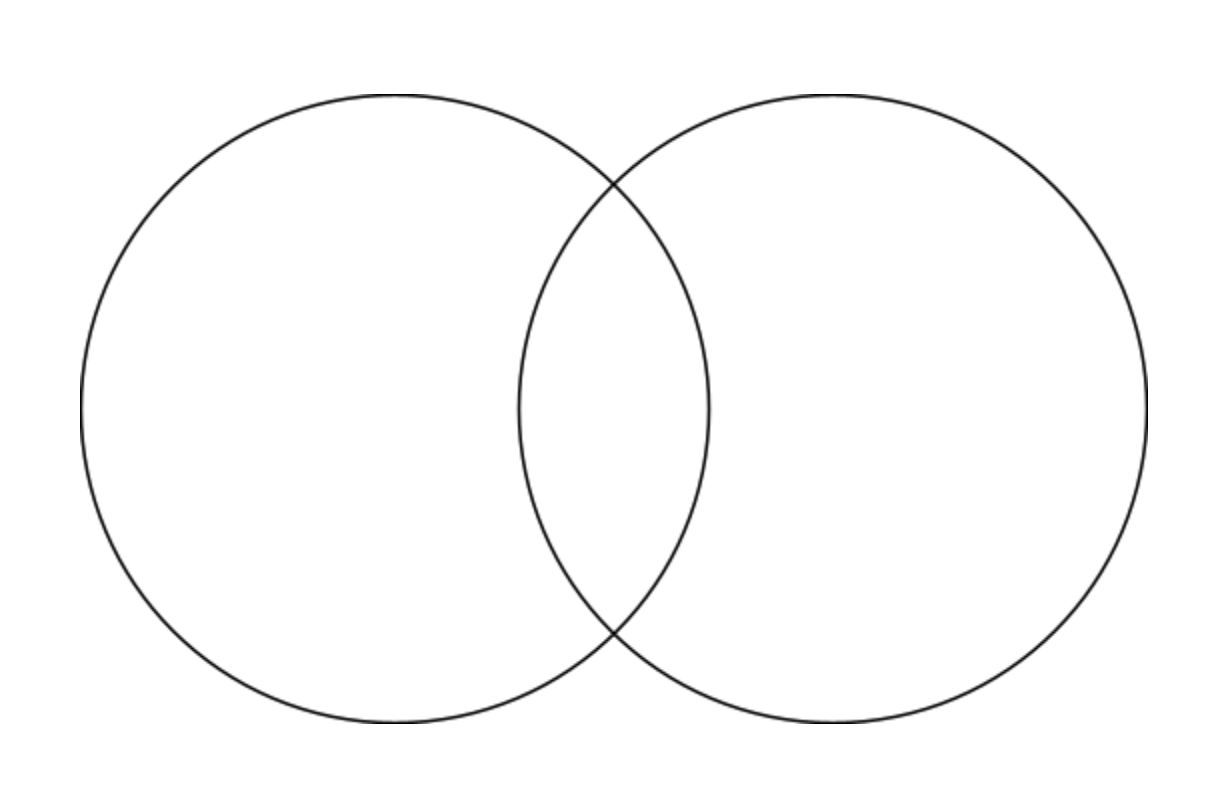
\includegraphics[width=0.6\textwidth]{venn-diagram}
    \centering
  \end{figure}

  In the above diagram, we assume the left circle corresponds to set $A$ and the
    right circle corresponds to $B$.
  The the possible sets we can make via the specified operators are:

  \begin{itemize}
    \item $A - B$, the left circle excluding the overlapping region.
    \item $A \cap B$, the overlapping region.
    \item $B - A$, the right circle excluding the overlapping region.
    \item $(A \cup B) \cap A$, the left circle.
    \item $(A \cup B) \cap B$, the right circle.
    \item $(A - B) \cup (B - A)$, the symmetric difference.
    \item $A \cup B$, the entire diagram.
  \end{itemize}

\end{proof}

\subsection{\verified{Exercise 4.19}}%
\label{sub:exercise-4.19}

Is $\powerset{(A - B)}$ always equal to $\powerset{A} - \powerset{B}$?
Is it ever equal to $\powerset{A} - \powerset{B}$?

\begin{proof}

  \lean{Bookshelf/Enderton/Set/Chapter\_2}
    {Enderton.Set.Chapter\_2.exercise\_4\_19}

  Let $A$ and $B$ be arbitrary sets.
  We show (i) that $\emptyset \in \powerset{(A - B})$ and (ii)
    $\emptyset \not\in \powerset{A} - \powerset{B}$.

  \paragraph{(i)}%
  \label{par:exercise-4.19-i}

    By definition of the \nameref{ref:power-set},
      $$\powerset{(A - B)} = \{ x \mid x \subseteq A - B \}.$$
    But $\emptyset$ is a subset of \textit{every} set.
    Thus $\emptyset \in \powerset{(A - B)}$.

  \paragraph{(ii)}%

    By the same reasoning found in \nameref{par:exercise-4.19-i},
      $\emptyset \in \powerset{A}$ and $\emptyset \in \powerset{B}$.
    But then, by definition of the relative complement,
      $\emptyset \not\in \powerset{A} - \powerset{B}$.

  \paragraph{Conclusion}%

    By the \nameref{ref:extensionality-axiom}, the two sets are never equal.

\end{proof}

\subsection{\verified{Exercise 4.20}}%
\label{sub:exercise-4.20}

Let $A$, $B$, and $C$ be sets such that $A \cup B = A \cup C$ and
  $A \cap B = A \cap C$.
Show that $B = C$.

\begin{proof}

  \lean{Bookshelf/Enderton/Set/Chapter\_2}
    {Enderton.Set.Chapter\_2.exercise\_4\_20}

  Let $A$, $B$, and $C$ be arbitrary sets.
  By the \nameref{ref:extensionality-axiom}, $B = C$ if and only if for all sets
    $x$, $x \in B \iff x \in C$.
  We prove both directions of this biconditional.

  \paragraph{($\Rightarrow$)}%

    Suppose $x \in B$.
    Then there are two cases to consider:

    \subparagraph{Case 1}%

      Assume $x \in A$.
      Then $x \in A \cap B$.
      By hypothesis, $A \cap B = A \cap C$.
      Thus $x \in A \cap C$ immediately implying $x \in C$.

    \subparagraph{Case 2}%

      Assume $x \not\in A$.
      Then $x \in A \cup B$.
      By hypothesis, $A \cup B = A \cup C$.
      Thus $x \in A \cup C$.
      Since $x \not\in A$, it follows $x \in C$.

  \paragraph{($\Leftarrow$)}%

    Suppose $x \in C$.
    Then there are two cases to consider:

    \subparagraph{Case 1}%

      Assume $x \in A$.
      Then $x \in A \cap C$.
      By hypothesis, $A \cap B = A \cap C$.
      Thus $x \in A \cap B$, immediately implying $x \in B$.

    \subparagraph{Case 2}%

      Assume $x \not\in A$.
      Then $x \in A \cup C$.
      By hypothesis, $A \cup B = A \cup C$.
      Thus $x \in A \cup B$.
      Since $x \not\in A$, it follows $x \in B$.

\end{proof}

\subsection{\verified{Exercise 4.21}}%
\label{sub:exercise-4.21}

Show that $\bigcup (A \cup B) = \bigcup A \cup \bigcup B$.

\begin{proof}

  \lean{Bookshelf/Enderton/Set/Chapter\_2}
    {Enderton.Set.Chapter\_2.exercise\_4\_21}

  Let $A$ and $B$ be arbitrary sets.
  By the \nameref{ref:extensionality-axiom}, the specified equality holds if and
    only if for all sets $x$,
    $$x \in \bigcup (A \cup B) \iff x \in \bigcup A \cup \bigcup B.$$
  We prove both directions of this biconditional.

  \paragraph{($\Rightarrow$)}%

    Suppose $x \in \bigcup (A \cup B)$.
    By definition of the union of sets, there exists some $b \in A \cup B$ such
      that $x \in b$.
    If $b \in A$, then $x \in \bigcup A$ and $x \in \bigcup A \cup \bigcup B$.
    Alternatively, if $b \in B$, then $x \in \bigcup B$ and
      $x \in \bigcup A \cup \bigcup B$.
    Regardless, $x$ is in the target set.

  \paragraph{($\Leftarrow$)}%

    Suppose $x \in \bigcup A \cup \bigcup B$.
    Then $x \in \bigcup A$ or $x \in \bigcup B$.
    WLOG, suppose $x \in \bigcup A$.
    By definition of the union of sets, there exists some $b \in A$ such that
      $x \in b$.
    But then $b \in A \cup B$ meaning $x$ is also a member of
      $\bigcup (A \cup B)$.

\end{proof}

\subsection{\verified{Exercise 4.22}}%
\label{sub:exercise-4.22}

Show that if $A$ and $B$ are nonempty sets, then
  $\bigcap (A \cup B) = \bigcap A \cap \bigcap B$.

\begin{proof}

  \lean{Bookshelf/Enderton/Set/Chapter\_2}
    {Enderton.Set.Chapter\_2.exercise\_4\_22}

  Let $A$ and $B$ be arbitrary, nonempty sets.
  By the \nameref{ref:extensionality-axiom}, the specified equality holds if and
    only if for all sets $x$,
    \begin{equation}
      \label{sub:exercise-4.22-eq1}
      x \in \bigcap (A \cup B) \iff x \in \bigcap A \cap \bigcap B.
    \end{equation}
  We prove both directions of this biconditional.

  \paragraph{($\Rightarrow$)}%

    Suppose $x \in \bigcap (A \cup B)$.
    Then for all $b \in A \cup B$, $x \in B$.
    In other words, for every member $b_1$ of $A$ and every member $b_2$ of $B$,
      $x$ is a member of both $b_1$ and $b_2$.
    But that implies $x \in \bigcap A$ and $x \in \bigcap B$.

  \paragraph{($\Leftarrow$)}%

    Suppose $x \in \bigcap A \cap \bigcap B$.
    That is, $x \in \bigcap A$ and $x \in \bigcap B$.
    By definition of the intersection of sets, forall sets $b$, if $b \in A$,
      then $x \in b$.
    Likewise, if $b \in B$, then $x \in b$.
    In other words, if $b$ is a member of either $A$ or $B$, $x \in b$.
    That immediately implies $x \in \bigcap (A \cup B$.

\end{proof}

\subsection{\partial{Exercise 4.23}}%
\label{sub:exercise-4.23}

Show that if $\mathscr{B}$ is nonempty, then
  $A \cup \bigcap \mathscr{B} = \bigcap\; \{A \cup X \mid X \in \mathscr{B} \}$.

\begin{proof}

  Refer to \nameref{sub:general-distributive-laws}.

\end{proof}

\subsection{\verified{Exercise 4.24a}}%
\label{sub:exercise-4.24a}

Show that if $\mathscr{A}$ is nonempty, then
  $\powerset{\bigcap\mathscr{A}} =
    \bigcap\; \{\powerset{X} \mid X \in \mathscr{A} \}$.

\begin{proof}

  \lean{Bookshelf/Enderton/Set/Chapter\_2}
    {Enderton.Set.Chapter\_2.exercise\_4\_24a}

  Suppose $\mathscr{A}$ is a nonempty set.
  Then $\bigcap \mathscr{A}$ is well-defined.
  Therefore
    \begin{align*}
      \powerset{\bigcap\mathscr{A}}
        & = \{ x \mid x \subseteq \bigcap \mathscr{A} \}
          & \textref{ref:power-set} \\
        & = \{ x \mid x \subseteq
          \{ y \mid \forall X \in \mathscr{A}, y \in X \} \}
          & \text{def'n intersection} \\
        & = \{ x \mid \forall t \in x,
          t \in \{ y \mid \forall X \in \mathscr{A}, y \in X \} \}
          & \text{def'n subset} \\
        & = \{ x \mid \forall t \in x,
          (\forall X \in \mathscr{A}, t \in X) \} \\
        & = \{ x \mid \forall X \in \mathscr{A},
          (\forall t \in x, t \in X) \} \\
        & = \{ x \mid \forall X \in \mathscr{A}, x \subseteq X \} \\
        & = \{ x \mid \forall X \in \mathscr{A}, x \in \powerset{X} \}
          & \textref{ref:power-set-axiom} \\
        & = \{ x \mid
          \forall t \in \{ \powerset{X} \mid X \in \mathscr{A} \}, x \in t \} \\
        & = \bigcap\; \{\powerset{X} \mid X \in \mathscr{A}\}.
    \end{align*}

\end{proof}

\subsection{\verified{Exercise 4.24b}}%
\label{sub:exercise-4.24b}

Show that
  \begin{equation}
    \label{sub:exercise-4.24b-eq1}
    \bigcup\; \{ \powerset{X} \mid X \in \mathscr{A} \} \subseteq
      \powerset{\bigcup\mathscr{A}}.
  \end{equation}
Under what conditions does equality hold?

\begin{proof}

  \lean{Bookshelf/Enderton/Set/Chapter\_2}
    {Enderton.Set.Chapter\_2.exercise\_4\_24b}

  We first prove \eqref{sub:exercise-4.24b-eq1}.
  Let $x \in \bigcup\; \{ \powerset{X} \mid X \in \mathscr{A} \}$.
  By definition of the union of sets,
    $(\exists X \in \mathscr{A}), x \in \powerset{X}$.
  By definition of the \nameref{ref:power-set}, $x \subseteq X$.
  By \nameref{sub:exercise-3.3}, $X \subseteq \bigcup \mathscr{A}$.
  Therefore $x \subseteq \bigcup \mathscr{A}$, proving
    $x \in \powerset{\mathscr{A}}$ as expected.

  \suitdivider

  \noindent
  We show $\powerset{\bigcup A} \subseteq 
    \bigcup\;\{ \powerset{X} \mid X \in \mathscr{A} \}$ if and only if
    $\bigcup\mathscr{A} \in \mathscr{A}$.

  \paragraph{($\Rightarrow$)}%

    Suppose $\powerset{\bigcup\mathscr{A}} \subseteq
      \bigcup\;\{ \powerset{X} \mid X \in \mathscr{A} \}$.
    By definition of the \nameref{ref:power-set},
      $\bigcup\mathscr{A} \in \powerset{\bigcup\mathscr{A}}$.
    By hypothesis, $\bigcup\mathscr{A} \in 
      \bigcup\;\{ \powerset{X} \mid X \in \mathscr{A} \}$.
    By definition of the union of sets, there exists some $X \in \mathscr{A}$
      such that $\bigcup\mathscr{A} \in \powerset{X}$.
    That is, $\bigcup\mathscr{A} \subseteq X$.
    But $\bigcup\mathscr{A}$ cannot be a proper subset of $X$ since
      $X \in \mathscr{A}$.
    Thus $\bigcup\mathscr{A} = X$.
    This proves $\bigcup\mathscr{A} \in
      \bigcup\;\{ \powerset{X} \mid X \in \mathscr{A} \}$.

  \paragraph{($\Leftarrow$)}%

    Suppose $\bigcup\mathscr{A} \in A$.
    Let $x \in \powerset{\bigcup\mathscr{A}}$.
    Since $\bigcup\mathscr{A} \in \mathscr{A}$, it immediately follows that
      $x \in \{\powerset{X} \mid X \in \mathscr{A}\}$.

  \paragraph{Conclusion}%

    Equality follows immediately from this fact in conjunction with the proof
      of \eqref{sub:exercise-4.24b-eq1}.

\end{proof}

\subsection{\verified{Exercise 4.25}}%
\label{sub:exercise-4.25}

Is $A \cup \bigcup \mathscr{B}$ always the same as
  $\bigcup\;\{ A \cup X \mid X \in \mathscr{B} \}$?
If not, then under what conditions does equality hold?

\begin{proof}

  \lean{Bookshelf/Enderton/Set/Chapter\_2}
    {Enderton.Set.Chapter\_2.exercise\_4\_25}

  We prove that
    \begin{equation}
      \label{sub:exercise-4.25-eq1}
      A \cup \bigcup \mathscr{B} =
        \bigcup\;\{ A \cup X \mid X \in \mathscr{B} \}
    \end{equation}
    if and only if $A = \emptyset$ or $\mathscr{B} \neq \emptyset$.
  We prove both directions of this biconditional.

  \paragraph{($\Rightarrow$)}%

    Suppose \eqref{sub:exercise-4.25-eq1} holds true.
    There are two cases to consider:

    \subparagraph{Case 1}%

      Suppose $B \neq \emptyset$.
      Then $A = \emptyset \lor \mathscr{B} \neq \emptyset$ holds trivially.

    \subparagraph{Case 2}%

      Suppose $B = \emptyset$.
      Then $$A \cup \bigcup \mathscr{B} = A \cup \bigcup \emptyset = A$$ and
        $$
          \bigcup\;\{ A \cup X \mid X \in \mathscr{B} \}
            = \bigcup \emptyset \\
            = \emptyset.
        $$
      Then by hypothesis \eqref{sub:exercise-4.25-eq1}, $A = \emptyset$.
      Then $A = \emptyset \lor \mathscr{B} \neq \emptyset$ holds trivially.

  \paragraph{($\Leftarrow$)}%

    Suppose $A = \emptyset$ or $\mathscr{B} \neq \emptyset$.
    There are two cases to consider:

    \paragraph{Case 1}%

      Suppose $A = \emptyset$.
      Then $A \cup \bigcup \mathscr{B} = \bigcup{\mathscr{B}}$.
      Likewise,
        $$
          \bigcup \{ A \cup X \mid X \in \mathscr{B} \}
            = \bigcup \{ X \mid X \in \mathscr{B} \} \\
            = \bigcup \mathscr{B}.
        $$
      Therefore \eqref{sub:exercise-4.25-eq1} holds.

    \paragraph{Case 2}%

      Suppose $B \neq \emptyset$.
      Then
        \begin{align*}
          A \cup \bigcup\mathscr{B}
            & = \{ x \mid x \in A \lor x \in \bigcup\mathscr{B} \} \\
            & = \{ x \mid x \in A \lor (\exists b \in \mathscr{B}) x \in b \} \\
            & = \{ x \mid (\exists b \in \mathscr{B}) x \in A \lor x \in b \} \\
            & = \{ x \mid (\exists b \in \mathscr{B}) x \in A \cup b \} \\
            & = \{ x \mid x \in \bigcup \{ A \cup X \mid X \in \mathscr{B} \} \\
            & = \bigcup \{ A \cup X \mid X \in \mathscr{B} \}.
        \end{align*}
      Therefore \eqref{sub:exercise-4.25-eq1} holds.

\end{proof}

\chapter{Relations and Functions}%
\label{chap:relations-functions}

\section{Ordered Pairs}%
\label{sec:ordered-pairs}

\subsection{\verified{Theorem 3A}}%
\label{sub:theorem-3a}

\begin{theorem}[3A]

  For any sets $x$, $y$, $u$, and $v$,
    \begin{equation}
      \label{sub:theorem-3a-eq1}
      \left< u, v \right> = \left< x, y \right> \iff u = x \land v = y.
    \end{equation}

\end{theorem}

\begin{proof}

  \lean{Bookshelf/Enderton/Set/Chapter\_3}
    {Enderton.Set.Chapter\_3.OrderedPair.ext\_iff}

  Let $x$, $y$, $u$, and $v$ be arbitrary sets.

  \paragraph{($\Leftarrow$)}%

    This follows trivially.

  \paragraph{($\Rightarrow$)}%

    Suppose $\left< u, v \right> = \left< x, y \right>$.
    Then, by definition of an \nameref{ref:ordered-pair},
      \begin{equation}
        \label{sub:theorem-3a-eq2}
        \{\{u\}, \{u, v\}\} = \{\{x\}, \{x, y\}\}.
      \end{equation}
    By the \nameref{ref:extensionality-axiom}, it follows
      $\{u\} \in \{\{x\}, \{x, y\}\}$ and
      $\{u, v\} \in \{\{x\}, \{x, y\}\}$.
    That is,
      $$\{u\} = \{x\} \quad\text{or}\quad \{u\} = \{x, y\}$$
      and
      $$\{u, v\} = \{x\} \quad\text{or}\quad \{u, v\} = \{x, y\}.$$
    There are 4 cases to consider:

    \paragraph{Case 1}%

      Suppose $\{u\} = \{x\}$ and $\{u, v\} = \{x\}$.
      The former identity implies $u = x$.
      The latter identity implies $u = v = x$.
      Then \eqref{sub:theorem-3a-eq2} simplifies to
        $$\{\{u\}\} = \{\{x\}, \{x, y\}\},$$ meaning $x = y$.
      Thus $v = y$ as well.

    \paragraph{Case 2}%

      Suppose $\{u\} = \{x\}$ and $\{u, v\} = \{x, y\}$.
      The former identity implies $u = x$.
      Substituting into the latter identity yields $\{u, v\} = \{u, y\}$.
      This holds if and only if $v = y$.

    \paragraph{Case 3}%

      Suppose $\{u\} = \{x, y\}$ and $\{u, v\} = \{x\}$.
      The former identity implies $x = y = u$.
      Substituting into the latter yields $\{u, v\} = \{u\}$.
      Thus $u = v$ which in turn implies $v = y$.

    \paragraph{Case 4}%
      Suppose $\{u\} = \{x, y\}$ and $\{u, v\} = \{x, y\}$.
      The former identity implies $x = y = u$.
      Substituting into the latter yields $\{u, v\} = \{u\}$.
      This implies $v = u$ which in turn implies $v = y$.

    \paragraph{Conclusion}%

      These cases are exhaustive and each implies that $u = x$ and $v = y$.

\end{proof}

\subsection{\verified{Lemma 3B}}%
\label{sub:lemma-3b}

\begin{theorem}[3B]

  If $x \in C$ and $y \in C$, then
    $\left< x, y \right> \in \powerset{\powerset{C}}$.

\end{theorem}

\begin{proof}

  \lean{Bookshelf/Enderton/Set/Chapter\_3}
    {Enderton.Set.Chapter\_3.theorem\_3b}

  Let $C$ be an arbitrary set and $x, y \in C$.
  Then, by definition of the \nameref{ref:power-set},
    $\{x\}$ and $\{x, y\}$ are members of $\powerset{C}$.
  Likewise, $\{\{x\}, \{x, y\}\}$ is a member of $\powerset{\powerset{C}}$.
  By definition of an \nameref{ref:ordered-pair},
    $\left< x, y \right> = \{\{x\}, \{x, y\}\}$.
  This concludes our proof.

\end{proof}

\subsection{\verified{Cartesian Product}}%
\label{sub:corollary-3c}
\label{sub:cartesian-product}

\begin{theorem}[3C]

  For any sets $A$ and $B$, there is a set whose members are exactly the
    pairs $\left< x, y \right>$ with $x \in A$ and $y \in B$.

\end{theorem}

\begin{proof}

  \lean*{Mathlib/SetTheory/ZFC/Basic}{Set.prod}

  \note{The above Lean proof is a definition (i.e. an axiom). It does not prove
    such a set's existence from first principles.}

  Define $C = A \cup B$.
  Then for all $x \in A$ and for all $y \in B$, $x$ and $y$ are both in $C$.
  By \nameref{sub:lemma-3b}, it follows that
    $\left< x, y \right> \in \powerset{\powerset{C}}$.
  The \nameref{ref:power-set-axiom} indicates $\powerset{\powerset{C}}$ is
    indeed a set.
  Therefore the \nameref{ref:subset-axioms} are applicable.
  This implies the existence of a set $D$ such that
    $$\forall z, (z \in D \iff z \in \powerset{\powerset{C}} \land
      (\exists x, \exists y, x \in A \land y \in B \land
        z = \left< x, y \right>)).$$
  By construction $D$ is the set whose members are exactly the pairs
    $\left< x, y \right>$ with $x \in A$ and $y \in B$.

\end{proof}

\section{Exercises 5}%
\label{sec:exercises-5}

\subsection{\verified{Exercise 5.1}}%
\label{sub:exercise-5.1}

Suppose that we attempted to generalize the Kuratowski definitions of ordered
  pairs to ordered triples by defining
  $$\left< x, y, z \right>^* = \{\{x\}, \{x, y\}, \{x, y, z\}\}.$$
Show that this definition is unsuccessful by giving examples of objects
  $u$, $v$, $w$, $x$, $y$, $z$ with
  $\left< x, y, z \right>^* = \left< u, v, w \right>^*$ but with either
  $y \neq v$ or $z \neq w$ (or both).

\begin{proof}

  \lean{Bookshelf/Enderton/Set/Chapter\_3}
    {Enderton.Set.Chapter\_3.exercise\_5\_1}

  Let $x = 1$, $y = 1$, and $z = 2$.
  Let $u = 1$, $v = 2$, and $w = 2$.
  Then
    \begin{align*}
      \left< x, y, z \right>^*
        & = \{\{x\}, \{x, y\}, \{x, y, z\}\} \\
        & = \{\{1\}, \{1, 1\}, \{1, 1, 2\}\} \\
        & = \{\{1\}, \{1, 2\}\}.
    \end{align*}
  Likewise
    \begin{align*}
      \left< u, v, w \right>^*
        & = \{\{u\}, \{u, v\}, \{u, v, w\}\} \\
        & = \{\{1\}, \{1, 2\}, \{1, 2, 2\}\} \\
        & = \{\{1\}, \{1, 2\}\}.
    \end{align*}
  Thus $\left< x, y, z \right>^* = \left< u, v, w \right>^*$ but $y \neq v$.

\end{proof}

\subsection{\verified{Exercise 5.2a}}%
\label{sub:exercise-5.2a}

Show that $A \times (B \cup C) = (A \times B) \cup (A \times C)$.

\begin{proof}

  \lean{Bookshelf/Enderton/Set/Chapter\_3}
    {Enderton.Set.Chapter\_3.exercise\_5\_2a}

  Let $A$, $B$, and $C$ be arbitrary sets.
  Then by definition of the \nameref{sub:cartesian-product} and union of sets,
    \begin{align*}
      A \times (B \cup C)
        & = \{ \left< x, y \right> \mid x \in A \land y \in (B \cup C) \} \\
        & = \{ \left< x, y \right> \mid
          x \in A \land (y \in B \lor y \in C) \} \\
        & = \{ \left< x, y \right> \mid
          (x \in A \land y \in B) \lor (x \in A \land y \in C) \} \\
        & = \{ \left< x, y \right> \mid (x \in A \land y \in B) \} \cup
          \{ \left< x, y \right> \mid (x \in A \land y \in C) \} \\
        & = (A \times B) \cup (A \times C).
    \end{align*}

\end{proof}

\subsection{\verified{Exercise 5.2b}}%
\label{sub:exercise-5.2b}

Show that if $A \times B = A \times C$ and $A \neq \emptyset$, then $B = C$.

\begin{proof}

  \lean{Bookshelf/Enderton/Set/Chapter\_3}
    {Enderton.Set.Chapter\_3.exercise\_5\_2b}

  Let $A$, $B$, and $C$ be arbitrary sets such that $A \neq \emptyset$.
  By definition of the \nameref{sub:cartesian-product},
    \begin{align}
      A \times B & = \{ \left< x, y \right> \mid x \in A \land y \in B \}
        & \label{sub:exercise-5.2b-eq1} \\
      A \times C & = \{ \left< x, y \right> \mid x \in A \land y \in C \}.
        & \label{sub:exercise-5.2b-eq2}
    \end{align}
  There are two cases to consider:

  \paragraph{Case 1}%

    Suppose $B \neq \emptyset$.
    Then $A \times B \neq \emptyset$ and $A \times C \neq \emptyset$.
    Let $\left< x, y \right> \in A \times B$.
    By \eqref{sub:exercise-5.2b-eq1}, $x \in A$ and $y \in B$.
    By the \nameref{ref:extensionality-axiom},
      $$\left< x, y \right> \in A \times B \iff \left< x, y \right> \in A \times C.$$
    Therefore $\left< x, y \right> \in A \times C$.
    By \eqref{sub:exercise-5.2b-eq2}, $x \in A$ and $y \in C$.
    Since membership of $y$ in $B$ and in $C$ holds biconditionally, the
      \nameref{ref:extensionality-axiom} indicates $B = C$.

  \paragraph{Case 2}%

    Suppose $B = \emptyset$.
    Then there is no $\left< x, y \right>$ such that $x \in A$ and $y \in B$.
    Thus $A \times B = \emptyset$ and $A \times C = \emptyset$.
    But then there cannot exist an $\left< x, y \right>$ such that $x \in A$
      and $y \in C$ either.
    Since $A \neq \emptyset$, it must be the case that $C = \emptyset$.
    Thus $B = C$.

\end{proof}

\subsection{\verified{Exercise 5.3}}%
\label{sub:exercise-5.3}

Show that $A \times \bigcup \mathscr{B} =
  \bigcup\;\{ A \times X \mid X \in \mathscr{B} \}$.

\begin{proof}

  \lean{Bookshelf/Enderton/Set/Chapter\_3}
    {Enderton.Set.Chapter\_3.exercise\_5\_3}

  Let $A$ and $\mathscr{B}$ be arbitrary sets.
  By definition of the \nameref{sub:cartesian-product} and the union of sets,
  \begin{align*}
    A \times \bigcup\mathscr{B}
      & = \{ \left< x, y \right> \mid
        x \in A \land y \in \bigcup\mathscr{B} \} \\
      & = \{ \left< x, y \right> \mid
        x \in A \land (\exists b \in \mathscr{B}), y \in b \} \\
      & = \{ \left< x, y \right> \mid
        (\exists b \in \mathscr{B}), x \in A \land y \in b \} \\
      & = \bigcup\; \{ A \times X \mid X \in \mathscr{B} \}.
  \end{align*}

\end{proof}

\subsection{\partial{Exercise 5.4}}%
\label{sub:exercise-5.4}

Show that there is no set to which every ordered pair belongs.

\begin{proof}

  For the sake of contradiction, suppose there exists a set $A$ to which every
    ordered pair belongs.
  That is, for all sets $x$ and $y$, $\left< x, y \right> = \{\{x\}, \{x, y\}\}$
    is a member of $A$.
  By the \nameref{ref:union-axiom}, it follows that $\bigcup\bigcup A$ is the
    set to which every set belongs.
  But \nameref{sub:theorem-2a} shows this is impossible.
  Thus our original assumption was wrong; there exists no set to which every
    ordered pair belongs.

\end{proof}

\subsection{\verified{Exercise 5.5a}}%
\label{sub:exercise-5.5a}

Assume that $A$ and $B$ are given sets, and show that there exists a set $C$
  such that for any $y$,
  \begin{equation}
    \label{sub:exercise-5.5a-eq1}
    y \in C \iff y = \{x\} \times B \text{ for some } x \text{ in } A.
  \end{equation}
In other words, show that $\{\{x\} \times B \mid x \in A\}$ is a set.

\begin{proof}

  \lean{Bookshelf/Enderton/Set/Chapter\_3}
    {Enderton.Set.Chapter\_3.exercise\_5\_5a}

  Let $a \in A$.
  By the \nameref{ref:pairing-axiom}, $\{a\}$ is a set.
  By \nameref{sub:cartesian-product}, $\{a\} \times B$ is a set.
  Again by the \nameref{ref:pairing-axiom}, $\{\{a\} \times B\}$ is a set.

  Next, by another application of \nameref{sub:cartesian-product}, $A \times B$
    is a set.
  By the \nameref{ref:power-set-axiom}, $\powerset{(A \times B)}$ is a set.
  Thus, by the \nameref{ref:subset-axioms}, the following is also a set:
    $$C = \{ y \in \powerset{(A \times B)} \mid
      \exists a \in A, \forall x, \left[ x \in y \iff
        \exists b \in B, x = \left< a, b \right> \right] \}.$$
  We now show that $C$ satisfies \eqref{sub:exercise-5.5a-eq1}.

  \paragraph{($\Rightarrow$)}%

    Suppose $y \in C$.
    Then there exists some $a \in A$ such that
      $$\forall x, \left[ x \in y \iff
        \exists b \in B, x = \left< a, b \right> \right].$$
    By the \nameref{ref:extensionality-axiom},
      \begin{align*}
        y
          & = \{ \left< a, b \right> \mid b \in B \} \\
          & = \{ \left< x, b \right> \mid x \in \{a\} \land b \in B \} \\
          & = \{ \{a\} \times B \}.
      \end{align*}

  \paragraph{($\Leftarrow$)}%

    Suppose $y = \{a\} \times B$ for some $a \in A$.
    By \nameref{sub:cartesian-product}, $x \in \{a\} \times B$ if and only if
      $\exists b \in B$ such that $x = \left< a, b \right>$.
    But then $x \in y$ if and only if $\exists b \in B$ such that
      $x = \left< a, b \right>$.
    This immediately proves $y \in C$.

\end{proof}

\subsection{\verified{Exercise 5.5b}}%
\label{sub:exercise-5.5b}

With $A$, $B$, and $C$ as above, show that $A \times B = \bigcup C$.

\begin{proof}

  \lean{Bookshelf/Enderton/Set/Chapter\_3}
    {Enderton.Set.Chapter\_3.exercise\_5\_5b}

  Let $A$ and $B$ be arbitrary sets.
  We want to show that
    \begin{equation}
      \label{sub:exercise-5.5b-eq1}
      A \times B = \bigcup\; \{\{x\} \times B \mid x \in A\}.
    \end{equation}
  The left-hand side of \eqref{sub:exercise-5.5b-eq1} is a set by virtue of
    \nameref{sub:cartesian-product}.
  The right-hand side of \eqref{sub:exercise-5.5b-eq1} is a set by virtue of
    \nameref{sub:exercise-5.5a}.
  We prove the set on each side is a subset of the other.

  \paragraph{($\subseteq$)}%

    Let $c \in A \times B$.
    Then there exists some $a \in A$ and $b \in B$ such that
      $c = \left< a, b \right>$.
    Thus $c \in \{a\} \times B$.
    We also note $\{a\} \times B \in \{\{x\} \times B \mid x \in A\}$,
      specifically when $x = a$.
    Therefore, by the \nameref{ref:union-axiom},
      $c \in \bigcup\;\{\{x\} \times B \mid x \in A\}$.

  \paragraph{($\supseteq$)}%

    Let $c \in \bigcup\; \{\{x\} \times B \mid x \in A\}$.
    By the \nameref{ref:union-axiom}, there exists some
      $b \in \{\{x\} \times B \mid x \in A\}$ such that $c \in b$.
    Then there exists some $x \in A$ such that $b = \{x\} \times B$.
    Therefore $c \in \{x\} \times B$.
    But $x \in A$ meaning $c \in A \times B$ as well.

  \paragraph{Conclusion}%

    Since we have shown
      $A \times B \subseteq \bigcup\; \{\{x\} \times B \mid x \in A\}$ and
      $A \times B \supseteq \bigcup\; \{\{x\} \times B \mid x \in A\}$, it
      follows \eqref{sub:exercise-5.5b-eq1} is a true identity.

\end{proof}

\section{Relations}%
\label{sec:relations}

\subsection{\verified{Theorem 3D}}%
\label{sub:theorem-3d}

\begin{theorem}[3D]

  If $\left< x, y \right> \in A$, then $x$ and $y$ belong to $\bigcup\bigcup A$.

\end{theorem}

\begin{proof}

  \lean{Bookshelf/Enderton/Set/Chapter\_3}
    {Enderton.Set.Chapter\_3.theorem\_3d}

  Let $A$ be a set and $\left< x, y \right> \in A$.
  By definition of an \nameref{ref:ordered-pair},
    $$\left< x, y \right> = \{\{x\}, \{x, y\}\}.$$
  By \nameref{sub:exercise-3.3}, $\{\{x\}, \{x, y\}\} \subseteq \bigcup A$.
  Then $\{x, y\} \in \bigcup A$.
  Another application of \nameref{sub:exercise-3.3} implies
    $\{x, y\} \subseteq \bigcup\bigcup A$.
  Therefore $x, y \in \bigcup\bigcup A$.

\end{proof}

\section{Exercises 6}%
\label{sec:exercises-6}

\subsection{\verified{Exercise 6.6}}%
\label{sub:exercise-6.6}

Show that a set $A$ is a relation iff $A \subseteq \dom{A} \times \ran{A}$.

\begin{proof}

  \lean{Bookshelf/Enderton/Set/Chapter\_3}
    {Enderton.Set.Chapter\_3.exercise\_6\_6}

  Let $A$ be a set.
  We prove the forward and reverse direction of the bidirectional.

  \paragraph{($\Rightarrow$)}%

    Suppose $A$ is a \nameref{ref:relation}.
    We show for all $a \in A$, $a \in \dom{A} \times \ran{A}$.
    Let $a \in A$.
    Since $A$ is a relation, $a$ is an ordered pair.
    Then there exists some sets $x$ and $y$ such that $a = \left< x, y \right>$.
    By the definition of the \nameref{ref:domain} and \nameref{ref:range} of
      $A$, $x \in \dom{A}$ and $y \in \ran{A}$.
    Thus $a = \left< x, y \right> \in \dom{A} \times \ran{A}$ as well.
    This proves $A \subseteq \dom{A} \times \ran{A}$.

  \paragraph{($\Leftarrow$)}%

    Suppose $A \subseteq \dom{A} \times \ran{A}$.
    Then for all $a \in A$, $a \in \dom{A} \times \ran{A}$.
    Therefore $a$ is an ordered pair.
    Since this holds for all $a \in A$, it follows $A$ is a relation.

\end{proof}

\subsection{\verified{Exercise 6.7}}%
\label{sub:exercise-6.7}

Show that if $R$ is a relation, then $\fld{R} = \bigcup\bigcup R$.

\begin{proof}

  \lean{Bookshelf/Enderton/Set/Chapter\_3}
    {Enderton.Set.Chapter\_3.exercise\_6\_7}

  Let $R$ be a \nameref{ref:relation}.
  We show that (i) $\fld{R} \subseteq \bigcup\bigcup R$ and (ii) that
    $\bigcup\bigcup R \subseteq \fld{R}$.

  \paragraph{(i)}%
  \label{par:exercise-6.7-i}

    Let $x \in \fld{R} = \dom{R} \cup \ran{R}$.
    That is, $x \in \dom{R}$ or $x \in \ran{R}$.

    If $x \in \dom{R}$, then there exists some $y$ such that
      $\left< x, y \right> = \{\{x\}, \{x, y\}\} \in R$.
    Then $\{x\} \in \bigcup R$ and $x \in \bigcup\bigcup R$.

    On the other hand, if $x \in \ran{R}$, then there exists some $t$ such that
      $\left< t, x \right> = \{\{t\}, \{t, x\}\} \in R$.
    Then $\{t, x\} \in \bigcup R$ and $x \in \bigcup\bigcup R$.

  \paragraph{(ii)}%
  \label{par:exercise-6.7-ii}

    Let $t \in \bigcup\bigcup R$.
    Then there exists some member $T \in \bigcup R$ such that $t \in T$.
    Likewise there exists some member $T' \in R$ such that $T \in T'$.
    By definition of a relation,
      $T' = \left< x, y \right> = \{\{x\}, \{x, y\}\}$ for some sets $x$ and
      $y$.
    Thus $t = x$ or $t = y$.
    By \nameref{sub:exercise-6.6}, $t \in \dom{R}$ or $t \in \ran{R}$.
    In other words, $t \in \fld{R}$.

  \paragraph{Conclusion}%

    Since \nameref{par:exercise-6.7-i} and \nameref{par:exercise-6.7-ii} hold,
      $\fld{R} = \bigcup\bigcup{R}$.

\end{proof}

\subsection{\verified{Exercise 6.8}}%
\label{sub:exercise-6.8}

Show that for any set $\mathscr{A}$:
  \begin{align}
    \dom{\bigcup{\mathscr{A}}}
      & = \bigcup\;\{ \dom{R} \mid R \in \mathscr{A} \},
      & \label{sub:exercise-6.8-eq1} \\
    \ran{\bigcup{\mathscr{A}}}
      & = \bigcup\;\{ \ran{R} \mid R \in \mathscr{A} \}.
      & \label{sub:exercise-6.8-eq2}
  \end{align}

\begin{proof}

  \statementpadding

  \lean*{Bookshelf/Enderton/Set/Chapter\_3}
    {Enderton.Set.Chapter\_3.exercise\_6\_8\_i}

  \lean{Bookshelf/Enderton/Set/Chapter\_3}
    {Enderton.Set.Chapter\_3.exercise\_6\_8\_ii}

  We prove (i) \eqref{sub:exercise-6.8-eq1} and then (ii)
    \eqref{sub:exercise-6.8-eq2}.

  \paragraph{(i)}%

    Let $x \in \dom{\bigcup{\mathscr{A}}}$.
    By definition of a domain, there exists some $y$ such that
      $\left< x, y \right> \in \bigcup{\mathscr{A}}$.
    By definition of the union of sets,
      $\exists y, \exists R \in \mathscr{A}, \left< x, y \right> \in R$.
    Equivalently,
      $\exists R \in \mathscr{A}, \exists y, \left< x, y \right> \in R$.
    By another application of the definition of a domain,
      $\exists R \in \mathscr{A}, x \in \dom{R}$.
    By another application of the definition of the union of sets,
      $x \in \bigcup\;\{ \dom{R} \mid R \in \mathscr{A} \}$.
    Since membership of these two sets holds biconditionally, it follows
      \eqref{sub:exercise-6.8-eq1} holds.

  \paragraph{(ii)}%

    Let $x \in \ran{\bigcup{\mathscr{A}}}$.
    By definition of a range, there exists some $t$ such that
      $\left< t, x \right> \in \bigcup{\mathscr{A}}$.
    By definition of the union of sets,
      $\exists t, \exists R \in \mathscr{A}, \left< t, x \right> \in R$.
    Equivalently,
      $\exists R \in \mathscr{A}, \exists t, \left< t, x \right> \in R$.
    By another application of the definition of a range,
      $\exists R \in \mathscr{A}, x \in \ran{R}$.
    By another application of the definition of the union of sets,
      $x \in \bigcup\;\{ \ran{R} \mid R \in \mathscr{A} \}$.
    Since membership of these two sets holds biconditionally, it follows
      \eqref{sub:exercise-6.8-eq2} holds.

\end{proof}

\subsection{\verified{Exercise 6.9}}%
\label{sub:exercise-6.9}

Discuss the result of replacing the union operation by the intersection
  operation in the preceding problem.

\begin{answer}

  \statementpadding

  \lean*{Bookshelf/Enderton/Set/Chapter\_3}
    {Enderton.Set.Chapter\_3.exercise\_6\_9\_i}

  \lean{Bookshelf/Enderton/Set/Chapter\_3}
    {Enderton.Set.Chapter\_3.exercise\_6\_9\_ii}

  Replacing the union operation with the intersection problem produces the
    following relationships
    \begin{align}
      \dom{\bigcap{\mathscr{A}}}
        & \subseteq \bigcap\;\{ \dom{R} \mid R \in \mathscr{A} \},
        & \label{sub:exercise-6.9-eq1} \\
      \ran{\bigcap{\mathscr{A}}}
        & \subseteq \bigcap\;\{ \ran{R} \mid R \in \mathscr{A} \}.
        & \label{sub:exercise-6.9-eq2}
    \end{align}

  We prove (i) \eqref{sub:exercise-6.9-eq1} and then (ii)
    \eqref{sub:exercise-6.9-eq2}.

  \paragraph{(i)}%

    Let $x \in \dom{\bigcap{\mathscr{A}}}$.
    By definition of the \nameref{ref:domain} of a set,
      $\exists y, \left< x, y \right> \in \bigcap{\mathscr{A}}$.
    By definition of the intersection of sets,
      $\exists y, \forall R \in \mathscr{A}, \left< x, y \right> \in R$.
    But this implies that
      $\forall R \in \mathscr{A}, \exists y, \left< x, y \right> \in R$.
    By another application of the definition of the \nameref{ref:domain} of a
      set, $\forall R \in \mathscr{A}, x \in \dom{R}$.
    By another application of the intersection of sets,
      $x \in \bigcap\;\{ \dom{R} \mid R \in \mathscr{A} \}$.
      Thus \eqref{sub:exercise-6.9-eq1} holds.

  \paragraph{(ii)}%

    Let $x \in \ran{\bigcap{\mathscr{A}}}$.
    By definition of the \nameref{ref:range} of a set,
      $\exists t, \left< t, x \right> \in \bigcap{\mathscr{A}}$.
    By definition of the intersection of sets,
      $\exists t, \forall R \in \mathscr{A}, \left< t, x \right> \in R$.
    But this implies that
      $\forall R \in \mathscr{A}, \exists t, \left< t, x \right> \in R$.
    By another application of the definition of the \nameref{ref:range} of a
      set, $\forall R \in \mathscr{A}, x \in \ran{R}$.
    By another application of the intersection of sets,
      $x \in \bigcap\;\{ \ran{R} \mid R \in \mathscr{A} \}$.
      Thus \eqref{sub:exercise-6.9-eq2} holds.

\end{answer}

\section{Exercises 7}%
\label{sec:exercises-7}

\subsection{\partial{Exercise 7.10}}%
\label{sub:exercise-7.10}

Show that an ordered $4$-tuple is also an ordered $m$-tuple for every positive
  integer $m$ less than $4$.

\begin{answer}

  Let $\left< x_1, x_2, x_3, x_4 \right>$ denote an arbitrary $4$-tuple.
  Then
    \begin{align}
      \left< x_1, x_2, x_3, x_4 \right>
        & = \left< \left< x_1, x_2, x_3 \right>, x_4 \right>
          & \label{sub:exercise-7.10-eq1} \\
        & = \left< \left< \left< x_1, x_2 \right>, x_3 \right>, x_4 \right>
          & \label{sub:exercise-7.10-eq2}
    \end{align}
  Here \eqref{sub:exercise-7.10-eq1} is an equivalent ordered $2$-tuple and
    \eqref{sub:exercise-7.10-eq2} is an equivalent ordered $3$-tuple.
  Furthermore, $\left< x_1, x_2, x_3, x_4 \right> =
    \left< \left< x_1, x_2, x_3, x_4 \right> \right>$, showing it can be
    represented as an ordered $1$-tuple as well.

\end{answer}

\section{Functions}%
\label{sec:functions}

\subsection{\verified{Theorem 3E}}%
\label{sub:theorem-3e}

\begin{theorem}[3E]

  For a set $F$, $\dom{(F^{-1})} = \ran{F}$ and $\ran{(F^{-1})} = \dom{F}$.
  For a relation $F$, $(F^{-1})^{-1} = F$.

\end{theorem}

\begin{proof}

  \statementpadding

  \lean*{Common/Set/Relation}
    {Set.Relation.dom\_inv\_eq\_ran\_self}

  \lean*{Common/Set/Relation}
    {Set.Relation.ran\_inv\_eq\_dom\_self}

  \lean{Common/Set/Relation}
    {Set.Relation.inv\_inv\_eq\_self}

  We prove that (i) $\dom{(F^{-1})} = \ran{F}$, (ii) $\ran{(F^{-1})} = \dom{F}$,
    and (iii) $(F^{-1})^{-1} = F$.

  \paragraph{(i)}%

    By definition of the \nameref{ref:domain}, $x \in \dom{(F^{-1})}$ if and
      only if there exists some $y$ such that $\left< x, y \right> \in F^{-1}$.
    By definition of the \nameref{ref:inverse} of a set,
      $\left< y, x \right> \in F$.
    By definition of the \nameref{ref:range}, $x \in \ran{F}$.
    Since each step holds biconditionally, it follows
      $\dom{(F^{-1})} = \ran{F}$ as expected.

  \paragraph{(ii)}%

    By definition of the \nameref{ref:range}, $x \in \ran{(F^{-1})}$ if and
      only if there exists some $t$ such that $\left< t, x \right> \in F^{-1}$.
    By definition of the \nameref{ref:inverse} of a set,
      $\left< x, t \right> \in F$.
    By definition of the \nameref{ref:domain}, $x \in \dom{F}$.
    Since each step holds biconditionally, it follows
      $\ran{(F^{-1})} = \dom{F}$.

  \paragraph{(iii)}%

    By definition of the \nameref{ref:inverse} of a set,
      \begin{align*}
        (F^{-1})^{-1}
          & = \{\left< u, v \right> \mid \left< v, u \right> \in F^{-1}\} \\
          & = \{\left< u, v \right> \mid \left< u, v \right> \in F\} \\
          & = F.
      \end{align*}

\end{proof}

\subsection{\verified{Theorem 3F}}%
\label{sub:theorem-3f}

\begin{theorem}[3F]

  For a set $F$, $F^{-1}$ is a function iff $F$ is single-rooted.
  A relation $F$ is a function iff $F^{-1}$ is single-rooted.

\end{theorem}

\begin{proof}

  \statementpadding

  \lean*{Common/Set/Relation}
    {Set.Relation.single\_valued\_inv\_iff\_single\_rooted\_self}

  \lean{Common/Set/Relation}
    {Set.Relation.single\_valued\_self\_iff\_single\_rooted\_inv}

  We prove that (i) any set $F$, $F^{-1}$ is a function iff $F$ is
    single-rooted and (ii) any relation $F$ is a function iff $F^{-1}$ is
    single-rooted.

  \paragraph{(i)}%
  \label{par:theorem-3f-i}

    Let $F$ be any set.

    \subparagraph{($\Rightarrow$)}%

      Suppose $F^{-1}$ is a \nameref{ref:function}.
      By definition, for each $x \in \dom{(F^{-1})}$, there is only one $y$
        such that $\left< x, y \right> \in F^{-1}$.
      By definition of the \nameref{ref:inverse} of $F$,
        $F^{-1} = \{\left< u, v \right> \mid vFu\}$.
      Then for each $x \in \ran{F}$, there exists exactly one $y$ such that
        $\left< y, x \right> \in F$.
      This definitionally means $F$ is single-rooted.

    \subparagraph{($\Leftarrow$)}%

      Suppose $F$ is single-rooted.
      By definition, for each $x \in \ran{F}$, there is only one $t$ such that
        $\left< t, x \right> \in F$.
      By definition of the \nameref{ref:inverse} of $F$,
        $F^{-1} = \{\left< u, v \right> \mid vFu\}$.
      Then for each $x \in \dom{(F^{-1})}$ there exists exactly one $t$ such
        that $\left< x, t \right> \in F^{-1}$.
      This definitionally means $F^{-1}$ is a function.

  \paragraph{(ii)}%

    Let $F$ be a \nameref{ref:relation}.

    \subparagraph{($\Rightarrow$)}%

      Suppose $F$ is a function.
      By \nameref{sub:theorem-3e}, $F = (F^{-1})^{-1}$.
      Then by \nameref{par:theorem-3f-i}, $F^{-1}$ is single-rooted.

    \subparagraph{($\Leftarrow$)}%

      Suppose $F^{-1}$ is single-rooted.
      Then by \nameref{par:theorem-3f-i}, $(F^{-1})^{-1}$ is a function.
      By \nameref{sub:theorem-3e}, $(F^{-1})^{-1} = F$.
      Thus $F$ is a function.

\end{proof}

\subsection{\verified{Lemma 1}}%
\label{sub:lemma-1}

For any one-to-one function $F$, $F^{-1}$ is also one-to-one.

\begin{proof}

  \lean{Common/Set/Relation}
    {Set.Relation.one\_to\_one\_self\_iff\_one\_to\_one\_inv}

  We prove that (i) $F^{-1}$ is a function and (ii) $F^{-1}$ is single-rooted.

  \paragraph{(i)}%
  \label{par:lemma-1-i}

    By hypothesis, $F$ is one-to-one.
    This means it is single-rooted, i.e. for all $x \in \ran{F}$, there exists
      exactly one $t$ such that $\left< t, x \right> \in F$.
    By definition of the \nameref{ref:inverse} of $F$,
      $\left< x, t \right> \in F^{-1}$.
    But then for all $x \in \dom{(F^{-1})}$, there exists exactly one $t$ such
      that $\left< x, t \right> \in F^{-1}$.
    Thus $F^{-1}$ is a function.

  \paragraph{(ii)}%
  \label{par:lemma-1-ii}

    By hypothesis, $F$ is single-valued.
    That is, for all $x \in \dom{F}$, there exists exactly one $y$ such that
      $\left< x, y \right> \in F$.
    By definition of the \nameref{ref:inverse} of $F$,
      $\left< y, x \right> \in F^{-1}$.
    But then for all $x \in \ran{(F^{-1})}$, there exists exactly one $y$ such
      that $\left< y, x \right> \in F^{-1}$.
    Thus $F^{-1}$ is single-rooted.

  \paragraph{Conclusion}%

    By \nameref{par:lemma-1-i} and \nameref{par:lemma-1-ii}, $F^{-1}$ is
      a one-to-one function.

\end{proof}

\subsection{\verified{Theorem 3G}}%
\label{sub:theorem-3g}

\begin{theorem}[3G]

  Assume that $F$ is a one-to-one function.
  If $x \in \dom{F}$, then $F^{-1}(F(x)) = x$.
  If $y \in \ran{F}$, then $F(F^{-1}(y)) = y$.

\end{theorem}

\begin{proof}

  \statementpadding

  \lean*{Bookshelf/Enderton/Set/Chapter\_3}
    {Enderton.Set.Chapter\_3.theorem\_3g\_i}

  \lean{Bookshelf/Enderton/Set/Chapter\_3}
    {Enderton.Set.Chapter\_3.theorem\_3g\_ii}

  Suppose $F$ is a one-to-one \nameref{ref:function}.
  Then \nameref{sub:lemma-1} indicates $F^{-1}$ is a one-to-one function with
    domain $\ran{F}$ and range $\dom{F}$.

  For all $x \in \dom{F}$, $\left< x, F(x) \right> \in F$.
  Then $\left< F(x), x \right> \in F^{-1}$.
  Since $F^{-1}$ is single-valued, $F^{-1}(F(x)) = x$.

  For all $y \in \ran{F}$, $\left< y, F^{-1}(y) \right> \in F^{-1}$.
  Then $\left< F^{-1}(y), y \right> \in F$.
  Since $F$ is single-valued, $F(F^{-1}(y)) = y$.

\end{proof}

\subsection{\partial{Theorem 3H}}%
\label{sub:theorem-3h}

\begin{theorem}[3H]

  Assume that $F$ and $G$ are functions.
  Then $F \circ G$ is a function, its domain is
    \begin{equation}
      \label{sub:theorem-3h-eq1}
      \{x \in \dom{G} \mid G(x) \in \dom{F}\},
    \end{equation}
    and for $x$ in its domain, $(F \circ G)(x) = F(G(x))$.

\end{theorem}

\begin{proof}

  Let $F$ and $G$ be \nameref{ref:function}s.
  By definition of the \nameref{ref:composition} of $F$ and $G$,
    \begin{equation}
      \label{sub:theorem-3h-eq2}
      F \circ G = \{\left< u, v \right> \mid \exists t(uGt \land tFv)\}.
    \end{equation}
  By construction, $F \circ G$ is a relation.
  By the definition of the \nameref{ref:domain} of a relation,
    $x \in \dom{(F \circ G)}$ if and only if there exists some $y$ such that
    $\left< x, y \right> \in F \circ G$.
  We prove that (i) $F \circ G$ is a function with domain satisfying
    \eqref{sub:theorem-3h-eq1}, and (ii) $(F \circ G)(x) = F(G(x))$.

  \paragraph{(i)}%
  \label{par:theorem-3h-i}

    By \eqref{sub:theorem-3h-eq2}, there exists some $t$ such that
      $\left< x, t \right> \in G$ and $\left< t, y \right> \in F$.
    Since $G$ is single-valued, $t$ is uniquely determined by $x$.
    Since $F$ is single-valued, $y$ is uniquely determined by $t$.
    Therefore, by transitivity, $y$ is uniquely determined by $x$.
    Thus $F \circ G$ is single-valued, i.e. $F \circ G$ is a function.

    Furthermore, by definition of function application, $t = G(x)$.
    Thus
      $$\left< x, G(x) \right> \in G \quad\text{and}\quad
        \left< G(x), y \right> \in F.$$
    This immediately implies \eqref{sub:theorem-3h-eq1} holds true.

  \paragraph{(ii)}%

    Let $x \in \dom{(F \circ G)}$.
    By definition, $\left< x, (F \circ G)(x) \right> \in F \circ G$.
    Then \eqref{sub:theorem-3h-eq2} implies $(F \circ G)(x)$ satisfies
      $\left< G(x), (F \circ G)(x) \right> \in F$.
    This is equivalent to saying $F(G(x)) = (F \circ G)(x)$ as expected.

\end{proof}

\subsection{\partial{Theorem 3I}}%
\label{sub:theorem-3i}

\begin{theorem}[3I]

  For any sets $F$ and $G$, $$(F \circ G)^{-1} = G^{-1} \circ F^{-1}.$$

\end{theorem}

\begin{proof}

  By definition of the \nameref{ref:composition} of $F$ and $G$,
    $$F \circ G = \{\left< u, v \right> \mid \exists t(uGt \land tFv)\}.$$
  By definition of the \nameref{ref:inverse} of a function,
    \begin{align*}
      (F \circ G)^{-1}
        & = \{\left< u, v \right> \mid \exists t (vGt \land tFu)\} \\
        & = \{\left< u, v \right> \mid \exists t (tFu \land vGt)\} \\
        & = \{\left< u, v \right> \mid
          \exists t \left[ u(F^{-1})t \land t(G^{-1})v \right]\} \\
        & = G^{-1} \circ F^{-1}.
    \end{align*}

\end{proof}

\subsection{\partial{Theorem 3J}}%
\label{sub:theorem-3j}

\begin{theorem}[3J]

  Assume that $F \colon A \rightarrow B$, and that $A$ is nonempty.
  \begin{enumerate}[(a)]
    \item There exists a function $G \colon B \rightarrow A$ (a "left inverse")
      such that $G \circ F$ is the identity function $I_A$ on $A$ iff $F$ is
      one-to-one.
    \item There exists a function $H \colon B \rightarrow A$ (a "right inverse")
      such that $F \circ H$ is the identity function $I_B$ on $B$ iff $F$ maps
      $A$ onto $B$.
  \end{enumerate}

\end{theorem}

\begin{proof}

  Let $F$ be a \nameref{ref:function} from nonempty set $A$ to set $B$.

  \paragraph{(a)}%

    We prove there exists a function $G \colon B \rightarrow A$ such that
      $G \circ F = I_A$ if and only if $F$ is one-to-one.

    \subparagraph{($\Rightarrow$)}%

      Suppose $G \colon B \rightarrow A$ is a function satisfying
        $G \circ F = I_A$.
      To prove function $F$ is one-to-one, it is sufficient to prove $F$ is
        single-rooted.
      Let $y \in \ran{F}$.
      Then there there exists some $x_1 \in \dom{F}$ such that $F(x_1) = y$.
      Suppose there exists another $x_2 \in \dom{F}$ such that $F(x_2) = y$.
      Then $G(F(x_1)) = G(y) = G(F(x_2))$.
      But $G \circ F = I_A$ so $x_1 = x_2$.
      Thus, for all $y \in \ran{F}$, there exists only one $x$ such that
        $\left< x, y \right> \in F$.
      That is, $F$ is single-rooted as expected.

    \subparagraph{($\Leftarrow$)}%

      Suppose $F$ is one-to-one.
      Then by \nameref{sub:lemma-1}, $F^{-1} \colon B \rightarrow A$ is also
        one-to-one.
      We show that $F^{-1} \circ F = I_A$.
      Let $x \in \dom{F}$.
      By \nameref{sub:theorem-3h}, $(F^{-1} \circ F)(x) = F^{-1}(F(x))$.
      By \nameref{sub:theorem-3g}, $F^{-1}(F(x)) = x$.
      Thus $F^{-1} \circ F = I_A$.

  \paragraph{(b)}%

    We prove there exists a function $H \colon B \rightarrow A$ such that
      $F \circ H = I_B$ if and only if $F$ maps $A$ onto $B$.

    \subparagraph{($\Rightarrow$)}%

      Suppose $H \colon B \rightarrow A$ is a function satisfying
        $F \circ H = I_B$.
      To prove $F$ maps $A$ onto $B$, we must prove $\ran{F} = B$.
      But for all $y \in B$, $F(H(y)) = y$.
      Thus $y \in \ran{F}$ meaning $B \subseteq \ran{F}$.
      Since $F$ maps $A$ into $B$ by hypothesis, $\ran{F} \subseteq B$.
      Thus $\ran{F} = B$ as expected.

    \subparagraph{($\Leftarrow$)}%

      Suppose $F$ maps $A$ onto $B$.
      That is, $\ran{F} = B$.
      We show that $F^{-1} \colon B \rightarrow A$ satisfies
        $F \circ F^{-1} = I_B$.
      Let $y \in \ran{F}$.
      By \nameref{sub:theorem-3h}, $(F \circ F^{-1})(y) = F(F^{-1}(y))$.
      By \nameref{sub:theorem-3g}, $F(F^{-1}(y)) = y$.
      Thus $F \circ F^{-1} = I_B$.

\end{proof}

\end{document}
